\documentclass{article}

\usepackage[OT1]{fontenc}
\usepackage{mathpazo}
\usepackage[english]{babel}

\usepackage{amsmath}
\usepackage{amsfonts}
\usepackage[utf8]{inputenc}
\usepackage{graphicx}
\usepackage{float}
\usepackage{hyperref}
\hypersetup{
    colorlinks,
    citecolor=black,
    filecolor=black,
    linkcolor=black,
    urlcolor=black
}

\title{\textbf{Artificial Intelligence}}
\author{Manuel Pagliuca}

\begin{document}

\maketitle
\tableofcontents
\newpage
\pagebreak
\section{Motivation}
Artificial neural networks are information processing systems, whose structure and
operation principles are inspired by the nervous system and the brain of animals and
humans.

Artificial neural networks are studied for various reasons.

\begin{itemize}
    \item Extracting knowledge from data (\textit{phenomena, events, processes, operating environment,...}).
    \item Understanding the phenomena that I’m observing, extracting the knowledge about that phenomena.
    \item Automated construction of computational paradigms for problem solving.
\end{itemize}

The ultimate goal is to be able to have a model which allow to describe the phenomenon
that I’m observing and using this model I would like to solve the specific application problem.

There is an huge variety of application, this is the reason which AI now is so popular, and we
have so many interested and expertise in this field.

The next evolution of the economy is based on availability of solution which are extracted
from the data by analyzing the data reasoning, the only problems is that our capability
of reasoning is limited by the fact that our brain is not able to analyze huge quantity
of data, with automated system we can exploit this and make more comprehensive models that describe
the process of systems we are observing and develop more accurate solutions.

Basically, artificial intelligence is mimicking the nature. We want to take the data
analyze the data make a model, and for doing this we use techniques, we want to enrich
the analysis we are doing through sensors from environments, we can use other
specific sets of techniques.

We have the need of putting together some ideas and observation, we can define rules for reasoning, we extract the knowledge,
but we can also build knowledge through reasoning. Basically, what we want to do is to try to replicate
how the living beings observe and operate in the environment, how express, interacts.

Not only but we want to observe how the individual evolves, population evolves, in order to understand the trend
of the environment. In this broad variety of approaches is to define some techniques which mainly are
in two big categories, from the point of view of intelligence :

\begin{itemize}
    \item \textbf{Symbolic approach}
    \item \textbf{Sub-symbolic approach}, which are sub-symbolic techniques for analyze the environment
          and the systems.
\end{itemize}

During this course we are focusing on sub-symbolic reasoning techniques:
\begin{itemize}
    \item \textbf{Neural networks}, which is a simulation of a living brain.
    \item \textbf{Fuzzy systems}, which embed the definition of quantities, which are fuzzy (not defined
          in a very crisp way).
    \item \textbf{Evolutionary computing}, which is a set of techniques which mimics the natural evolution of the
          species so we can try to optimize the solution by using the basic concept of the natural evolution of the species.
\end{itemize}


\section{Neural networks}
\subsection{Biological background}
Basically, the aim of the artificial neural networks in \textit{mimicking} the behavior of our brain starts
from the fields of neural biology and neural physiology. What this discipline tries to do is to analyze the
behavior of the biological neurons cells and understand how they behave for retrieving
the information from the outer world.

The neurons use sensors and special cells to connect to the external world and get information.
As humans or other biological species, we have five senses, taking for example the eyes, they are receptors
which are able to see what a round us is, they are able to reconstruct the scene we got around us.

Basically, with artificial neural networks we are trying to replicate what \textbf{biology} does for us, in neurobiology
we build a model of what is happening in the neurons, this model describes how the neurons are
interacting together to extract the knowledge, to build memory, construct reasoning, take decisions.

In computer science we want to build this model in computer just for trying to do something similar, we want to mimic the
behavior of the natural brain in order to try to replicate in an artificial environment the same operation.

We are building the \textit{model} for neurons in the computer, in this way we are able to use these
artificial models to \textit{learn} the environment and to solve practical problem (predict possible behaviors
and solve optimization problem, like we do naturally). We also have some basis in other disciplines like
physics and chemistry since we may want to use the neural networks, also for describing physical phenomena,
not only to create reasoning in our mind but we want to create models of phenomena, this can be used for various application.
We can create an abstract model, and instead of observing the real world we can observe how the model behave in some conditions.

Neural networks and in general artificial intelligence, is a discipline of computer science and
engineering, then we use some inspirations from other discipline but the core of the theoretical aspect
of the foundation which defines the artificial neural networks this is an area which is been to computer science and engineering.
\subsection{Reasons for studying the biological background}
The reasons for studying the BB (\textit{biological background}) in computer science are two:
\begin{itemize}
    \item The \textbf{first reason} for studying the neural networks is the fact that they are a very appealing model,
          since they work in \textbf{parallel} means that they have an intrinsically extremely high \textit{parallel process capability}.
          This is why computer scientist are so attracted to this topic. Our brain in many cases find the solution immediately, this
          is fascinating, this happens because we are exploiting the parallel capability of our neural networks.
    \item The \textbf{second reason} why we are studying this technology is the fact that there is really a huge amount of \textit{practical
              application} in broad variety of area : \textit{industrial manufactory, products medicine, finances, economy, social networks, data analysis, ...}
\end{itemize}

\subsection{Neurons}
\begin{figure}[H]
    \centering
    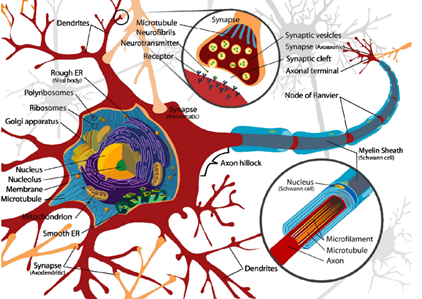
\includegraphics[width=10cm]{images/neuron1.png}
    \caption{Neuron}
    \label{fig:neurone_1}
\end{figure}

The \textit{central} part of the neuron is the part, which is managing the entire cell, this core the
nucleus is listening what is happening around the neuron,
when I have a \textbf{solicitation} from the external (other neurons or special cells related to the five senses).

When there is sufficient stimulation coming from this cells the nucleus is solicited and at a given
point the nucleus realizes that the solicitation is so high that he has to
take an \textbf{action}, the action is to send a \textit{signal} around the \textit{axon} (the long extension covered in blue),
this will lead to have a \textit{polarization} of an \textit{electric signal} which is flowing along this connection
and this will reach other neurons that are connected to the end of the axon to the synapses.

\begin{figure}[H]
    \centering
    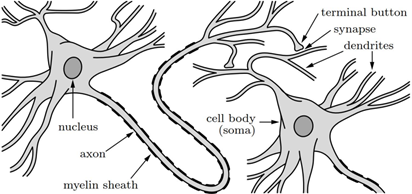
\includegraphics[width=10cm]{images/neuron2.png}
    \caption{Connection between two neurons}
    \label{fig:neurone_2}
\end{figure}

The \textbf{axon} is covered by an appropriate \textit{protein} (covered in blue) which protect the axon itself,
and make sure that the polarization that occur on the nucleus is transmitted along the axon so that this signal is able
to reach the synapse.

Basically, what we see is that the \textbf{neuron is exciting the nucleus}, which is generating the excitation along the axon,
then it will reach the terminal synapses.

Each synapse is connected to the synapses of \textit{another} neuron, so that the signals which are generated by
the nucleus and sent to the axon and then to the synapsis terminal at the terminal the synapses
are releasing some chemicals called \textbf{neurotransmitters}.

These \textit{substances} are exciting the synapses of the connected neuron, bu stimulating the synapses this excitation is
propagated from the \textbf{dendrites} to the nucleus of the other neuron, when the other cell is \textit{sufficiently excited} by
from the amount of stimulation generated by the neurotransmitter the nucleus will generate again a new stimulation
which is going along the axon and reach another neuron (and so on...).

The axon is \textit{depolarized} if there is enough excitatory input, basically this is how the signals are propagated
through the brain.

Due to the fact that each neuron can stimulate each other neurons connected to them,
this will create the \textbf{parallel processing} in our brain, so that each component will take care
of analyzing each part of the information and this is a consequence to derive a part of the total computation.

\subsection{Computer vs Human brain}
When we look to the differences between a computer and the human brain what we notice,
is that in the computer we got processors composed by many \textit{transistors}, the human brain counterpart
the got $10^11$ \textit{neurons}, the number of the latter overcomes the number of the cores in a processor.

The neurons aren’t able to process the same \textit{complex operation} of a core, but they are still so many that they
can overcome the limit of the complexity of the individual operation with the fact that they are working significantly in
parallel.

\begin{figure}[H]
    \centering
    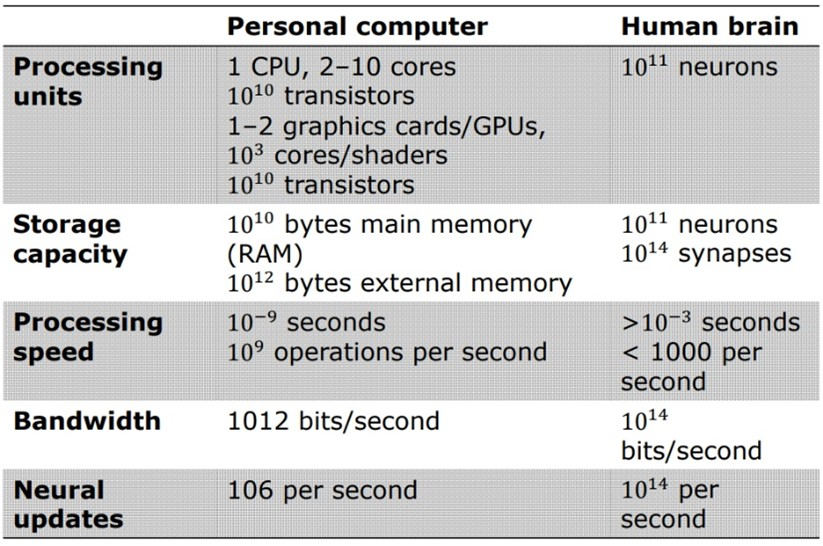
\includegraphics[width=10cm]{images/tab_pc_vs_brain.jpg}
    \caption{PC vs Human brain}
    \label{fig:tab_pc_vs_brain}
\end{figure}

The \textbf{storage} of the neurons has an immense storage potential than any other memory capacity. The \textbf{processing speed}
seems \textit{much higher} on the computer, but the parallel operation that you can do in parallel in the human brain in
the end \textit{overcome} the processing speed of the hardware of a computer.

Basically, what we can observe is that the biological neural networks are able to outperform significantly the processor that
we have nowadays, there are some researches carried out which are trying to create processors which are replicating in
hardware the operation of the biological neural networks but still the capabilities of this systems are \textit{far} from the
capability of human brain.

It may \textit{seem} in some system that they are working faster then humans, it may seem that they are running better, but actually
what you have is that you have the ability in the computer to run the algorithms and the explore the
possible (deterministic) moves in a fast way but needs some background knowledge
in order to that in a very short time.

Advantages of biological neural network:
\begin{itemize}
    \item High processing speed due to massive parallelism.

    \item Even if we have a significant amount of the biological neural network damaged, the system is
          considered \textbf{fault tolerance}, it remains functional even if larger parts of the network get \textit{damaged} (maybe some functions will be disabled).
          The other cells are able to overcome the death cells, this thanks to the elasticity of the neurons which are able
          to overcome possible damages in the structures.

    \item If more neurons are failing, the brain will \textit{degrade the performances} in a \textit{graceful way},
          it will not just stop working, will work a bit less not with the same performance and the same functionality
          but with reduced function. Only when a \textit{really massive} number of neurons is dying at that point a
          function is not working anymore.

    \item They are well suited for inductive learning (\textit{learning from examples, generalization from instances}).
\end{itemize}

What we are trying to do with artificial neural networks is to capture the parallel operation of the brain. The ability to
extract the knowledge from the data, we want to replicate these capabilities.

There are some problems due to the \textbf{ANN} (artificial neural networks), if we kill part of the architecture which
is replicating the \textbf{BNN} (biological neural networks), the ANN is \textbf{not automated to survives}, we have to
assure some physical redundance, this is a problem of the architecture we are using to execute the computation of the ANN.

What we want to do in our model is to construct a \textit{set of abstract models of the neurons} that we call
\textbf{artificial neurons}, and we like to connect them together to replicate the structure that we have in the
natural brain this is why we have the ANN, a connection of neurons that is trying to mimic the behavior of the brain.

The complexity of the brain is so high that is actually difficult to replicate everything in ANN,
what we are doing is to replicate a specific function of the brain which is able to solve a specific application
problem that we have.

\subsection{Threshold Logic Units}
This is the first \textit{abstract model} for an artificial neuron of the brain.
A \textbf{threshold logic unit} (TLU) is a \textit{processing unit} (neuron) with several inputs.
It can solve a very simple set of problems.

We have a \textbf{core} (the neuron) with several \textit{inputs} that are reaching the neuron, and we have the
\textit{output} which is delivered to the subsequential neurons which are connected with it.
A TLU is a processing unit in which the output is governed by a threshold $\theta$, if it has a \textit{sufficient excitation}
from the inputs, then the TLU became \textbf{active} (value $1$) and generates the output $y$.

\begin{figure}[H]
    \centering
    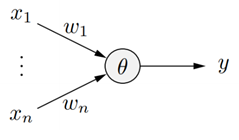
\includegraphics[width=6cm]{images/tlu.png}
    \caption{Threshold logic unit}
    \label{fig:tlu}
\end{figure}

We have $n$ inputs identified by $x_1,...,x_n$ the unit is generating only one output $y$ each input is \textbf{not}
delivered directly to the core of the TLU, but each input is \textbf{weighted}, some are more relevant,
and others are less relevant (exactly how we are doing when we consider the data from the external world).

\begin{figure}[H]
    \centering
    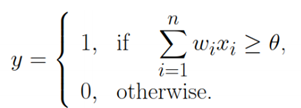
\includegraphics[width=6cm]{images/tlu_working_system.png}
    \caption{TLU conditions}
    \label{fig:tlu_conditions}
\end{figure}

This means that our problem is depending on the most important information, this is what happens in the real world.

In the ANN we are replicating the relevance of the individual input, we can control how much each input is actually
important to influence the generation of the output, to do this we use a weight $w$ for each of the input so
that the TLU will not see exactly the input but will see a weighted input, this will allow the modulation of
each input by giving to each of them the appropriate importance during the generation of the final output.

When the TLU is solicited enough it will generate an output $y$ that will be delivered to the \textit{terminal synapse}
to another neuron.
\begin{itemize}
    \item If the \textbf{excitation is enough}, mathematically means that the weighted summation is greater
          than a thresh $\theta$, we generate $1$ (the neuron is active).
    \item If the \textbf{excitation is not enough} for overcoming the threshold $\theta$, we generate $0$.
\end{itemize}

This model that tries to represent what is happening in the BNN from two scientists, also called the \textbf{McCulloch-Pitts neuron}.
\subsubsection{Conjunction example}
The result is equal to $1$ only when the two outputs are equal to $1$.
There is not a standard way to select the threshold $\theta$, we have to choose that in base of the
function that we want to implement. In this case I have to select a $\theta$ which is greater than the biggest weight.

$$x_1\land x_2$$

\begin{figure}[H]
    \centering
    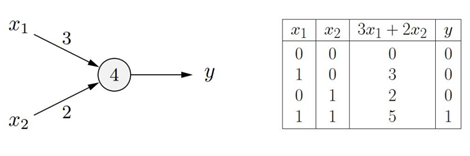
\includegraphics[width=10cm]{images/conj_TLU.png}
    \caption{Conjunction TLU}
    \label{fig:tlu_conjunction}
\end{figure}

\subsubsection{Implication example}
I can choose the value of the threshold in order to have the proper function, in this case applies on the same ways.
\textit{How can I choose the interconnection weights?}

The problem is that there are no general rules, I choose the weights according to the intrinsic relevance of each
input variable.

\textit{How can I do that when we have a high number of inputs?} we will see that there is a procedure for doing that.
$$x_2\rightarrow x_1$$
\begin{figure}[H]
    \centering
    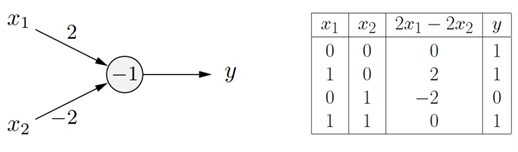
\includegraphics[width=10cm]{images/impl_TLU.png}
    \caption{Implication TLU}
    \label{fig:tlu_implication}
\end{figure}

\subsubsection{Multiple inputs example}
In this case we can see that we have three possible inputs, we can discriminate the
inputs in excitatory input and inhibitory input. The first tries to contributes
to the final computation of the neuron in such a way that the results
will be greater than the threshold, the other neuron does the opposite.

\begin{figure}[H]
    \centering
    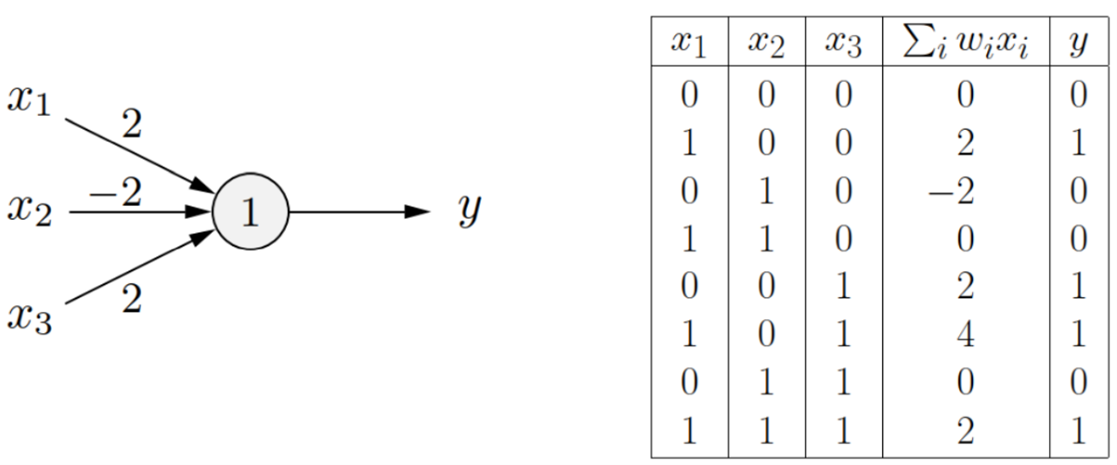
\includegraphics[width=10cm]{images/complex_TLU.png}
    \caption{Three-input TLU}
    \label{fig:tlu_3_input}
\end{figure}

\subsection{Geometric interpretation}
The geometric interpretation is significantly helpful to derive a \textit{method} to
configure the threshold and the weights starting from the data. We will consider a
single and simple TLU, we will try to understand how we can interpret the
behavior of the TLU in a geometrical way.

You know that is possible to represent a straight line on a plane in any of
the following forms :
\begin{figure}[H]
    \centering
    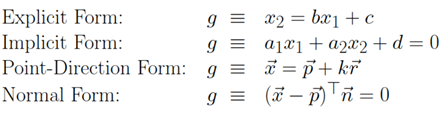
\includegraphics[width=10cm]{images/geom_interp.png}
    \caption{Different form for representing a straight line}
    \label{fig:line_repr}
\end{figure}

If i \textbf{implicit form}, where you have a weighted combination of the two variables plus a
possible threshold, a vector representation in point-direction form and normal form.
Any of this is fine to represent a straight line in the plane, we are considering just
two variables $x_1$ and $x_2$, and use one of the many representations.

\begin{figure}[H]
    \centering
    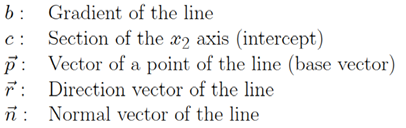
\includegraphics[width=9cm]{images/geom_interp_impl.png}
    \caption{Implicit form representation legend}
    \label{fig:line_impl_form_legend}
\end{figure}

\begin{figure}[H]
    \centering
    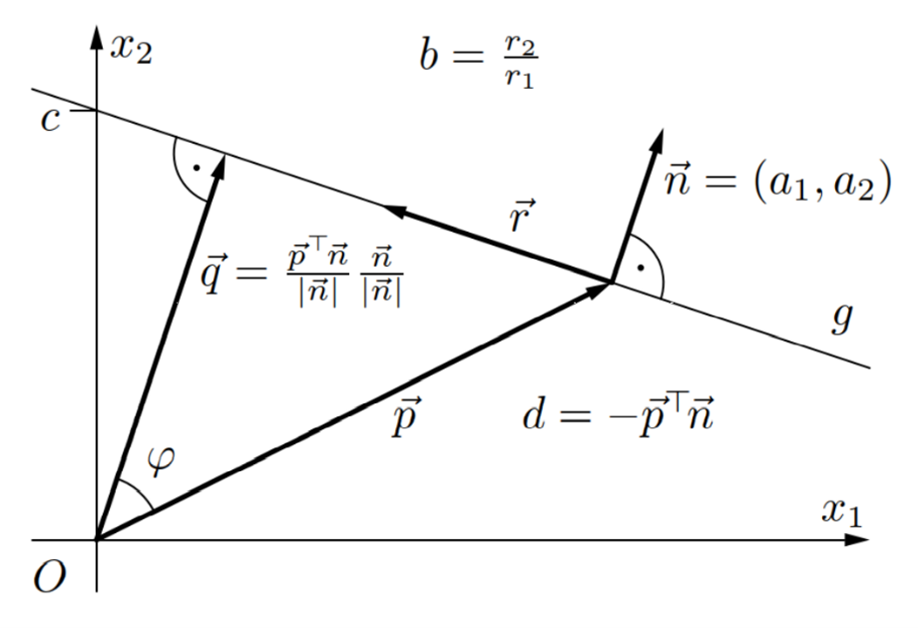
\includegraphics[scale=1]{images/geom1.png}
    \label{fig:geom_1}
\end{figure}

In the case of the \textit{explicit/implicit form} the $\vec{b}$ is the \textbf{inclination}
(or \textit{gradient}) of the straight line in respect of the horizontal axis,
and $c$ is the intercept of the vertical axis.

If we look to the normal $\vec{n}$ we want to pick the vector which is \textit{orthogonal}
to the straight line. The straight line is represented by all the points which starts from the
origin and has a quantity in the direction of the normal. The vector $\vec{p}$ identifies a
point in the example, we consider that point belonging to our straight line,
the distance of the straight line respect to the origin $O$ is given by $|\vec{q}|$ which is
the projection of $\vec{p}$ on straight line $g$.

\begin{figure}[H]
    \centering
    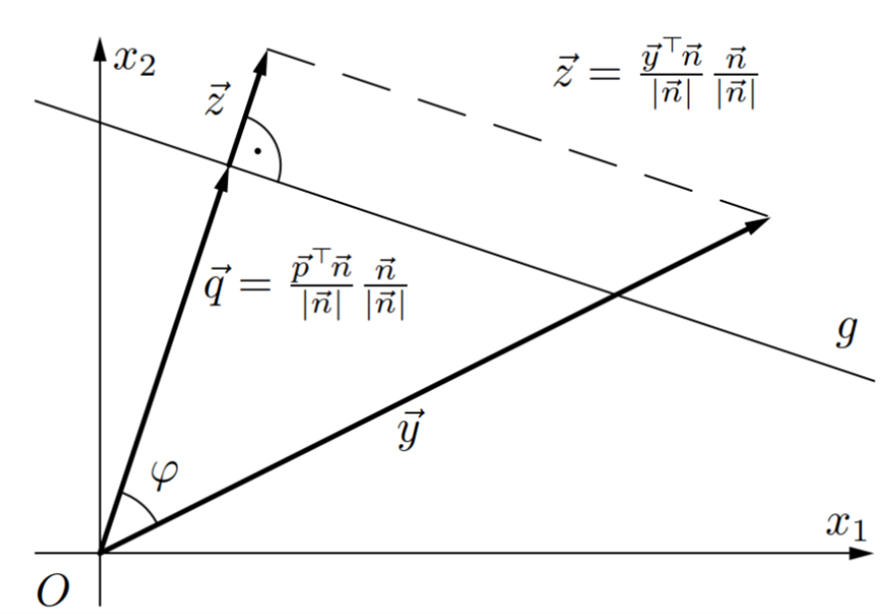
\includegraphics[scale=1]{images/geom2.png}
    \label{fig:geom_2}
\end{figure}

Considering this other graphical representation it is possible to know on which side
a points lands. If we take the vector representing $\vec{y}$ a point,
and i compute the projection in the direction of the normal, the projection
of this is the vector $\vec{z}$.

To understand on which side the points are, i just need to see if the vector $\vec{z}$ (which is the
projection of our point) is shorter or longer than the point i observe on the straight line, which
is pointed by $\vec{q}$. This means that all points (expressed by a vector) which have a \textbf{module}
higher then the projected point onto the straight line ($\vec{q}$), are part of the plane above the
straight line (they will \textit{satisfies} the solution), viceversa, they will be below the plane if the
module will be shorter then $\vec{q}$ (they won't satisfy the condition).

Basically the straight line which defines the behavior of my TLU, splits the plane in two parts (since i'm
considering only $x_1$ and $x_2$). All the points which distance is greater then

\begin{figure}[H]
    \centering
    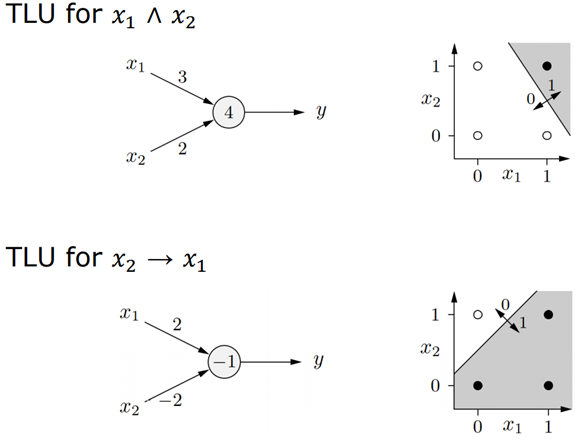
\includegraphics[scale=0.8]{images/tlu_examples_interp.png}
    \caption{Solution of the \textit{conjunction} and \textit{bi-implication}}
    \label{fig:example_interp}
\end{figure}

Now Let’s go back to the two examples that we have seen before,
starting with the conjunction, in this means that I have three points in which the output
has to be $0$, and one point where the result is $1$. This means that if I represent the straight
line with $x_1=3$, $x_2=3$ and the intercept equal to $4$ i will draw a line which is actually
separating in a clear way the element in which the output is equal to $1$ from the values
where the output is equal to $0$.
\newline
\newline
For the case of three variables, this is more complex, we need to generalize this idea moving from
a plane to a three-dimensional space. Think about the three axis and look at the combination of the
dots, you need to set a plane, so you have to separate one set of inputs for which the output has
to be equal to $1$ from the set of inputs combinations where the output is equal to $0$.

\begin{figure}[H]
    \centering
    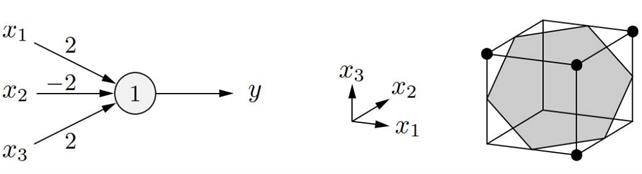
\includegraphics[scale=0.6]{images/three_input_sol_example.png}
    \caption{Solution of the complex TLU}
    \label{fig:example_three_sol}
\end{figure}

Basically, if you represent the plane using these information’s you will have this
kind of plane (that looks like a hexagon) dividing the solution from the $0$ values.

\textit{So how we choose the threshold and interconnection weights?} I have to look at geometrical
distribution of the points for the combination of the input which the output must be equal to $1$
and the one where the output must be equal to $0$, I have to take a straight line or plane and I
need to position the divisor in a way that I clearly separate the two groups. If I can do that,
that set of values (inputs and threshold) are the one that I need to use in my ANN.

\begin{figure}[H]
    \centering
    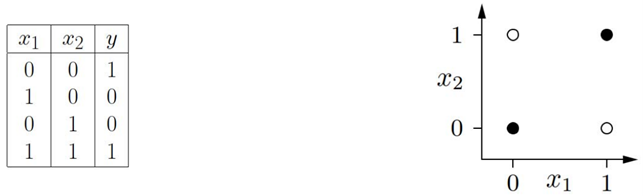
\includegraphics[scale=0.6]{images/bi_implic_no_sol.png}
    \caption{The bi-implication problem}
    \label{fig:bi-impl-problem}
\end{figure}

Let’s analyze another example, the bi-implication problem, this problem results in this kind of
distribution in the plane, as you can see it is not possible to separate these points with a
straight line. As a consequence, we don’t have any TLU for solving this problem, even if this is
a simple problem. We have to introduce some notions for understanding the reasons behind
this problem.
\subsubsection{Linear separability}
Two set of points in the \textbf{Euclidean Space}, consider $x_1, x_2,...,x_n$ as the variable for
the TLU, since we have n possible inputs you are analyzing a problem represented in $n$
dimensional Euclidean space.

If you have in this Euclidean space two set of points they are \textbf{linearly separable},
if and only if there exists at least one point, line, plane or hyperplane, such that all
points of the first set lie on one side and all points of the other set lie on the
other side of this point, line, plane or hyperplane.

The point sets can be separated by a linear decision function.

If you are in a mono dimensional space you have one input only,
your Euclidean Space is a line, you have one point on this straight line which is separating
your space the line in two parts, the output is one, for the other point the output is $0$.
If you have a plane, we have two input variables, we have to find a plane that separates
the two sets of points.
\subsubsection{Convex hull}
A set of points in the Euclidean Space is called \textbf{convex} if it is non-empty and
connected and for every pair of points in it every point on the straight-line segment
connecting the points of the pair is also in the set.

A \textbf{convex hull} of a set of points $X$ in a Euclidean Space is the smallest convex set of
points that contains $X$. Alternatively, the convex hull of a set of points $X$ is the intersection
of all convex sets that contain $X$.
\subsection{Solution of the bi-implication problem}
Two sets of points in Euclidean Space are linearly separable if and only if their convex hulls
are disjoint. In the bi-implication problem, the convex hulls are the diagonal line segments.

They share their intersection point and this means that they are not disjoint, therefore
the double implication is not linearly separable.

\begin{figure}[H]
    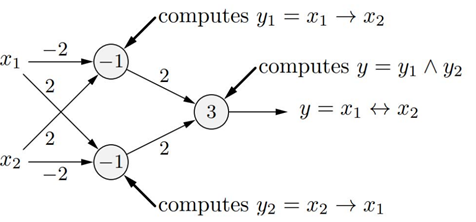
\includegraphics[scale=0.8]{images/sol_bi_implic_problem.png}
    \centering
    \caption{TLUs to the bi-implication problem}
\end{figure}
What we can do is putting together more neurons to try to address more complex problem where
one neuron can’t solve. We are creating a network of TLUs, we are splitting the problem in two
sub problems.

The problem of implication can be solved with a single TLU, we create a more complex structure
in which are able to solve the problem.

Let’s see what happens geometrically, the two points $a$ and $c$, are going to be separated
from the first two  TLUs, I set one of the TLU so that all points which are below the straight
line represented by $g_2$ fives and output equal to $1$, and then i set a second straight line
represented by $g_1$ where all points are all over the straight line the values are equal to $1$,
and then I merge this information.

\begin{figure}[H]
    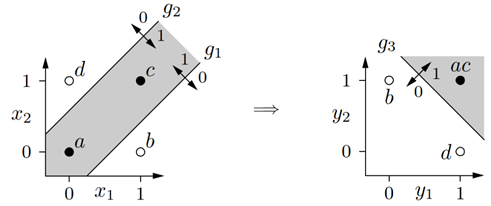
\includegraphics[scale=0.8]{images/sol_bi_implic_problem_graph.png}
    \centering
    \caption{Solution of the bi-implication problem}
\end{figure}

I combine these information from the previous group in the third neuron so that I transform
the representation of the information, I can merge the information of the points $a$ and $c$,
so that both the output of the two TLU is equal to $1$ is represented by one points (in this case
they are the same) and then I have the two other points $b$ and $d$ which are in both the parts
above and below the line, for them the solicitation is not enough to generate an output
equal to $1$, as a consequence I obtained a linear separability.

I transformed the stripe in a semi plane with the third TLU, which identifies the linear
separability, I don’t have that propriety only with the first TLU but also with the second,
both TLUs allow me to partition the first space in three parts.

\subsection{Arbitrary boolean functions}
I can work with any arbitrary \textbf{Boolean function}; in this example I have a
Boolean function of three variables. I have these values of the value $y$ according to the formula.

\begin{figure}[H]
    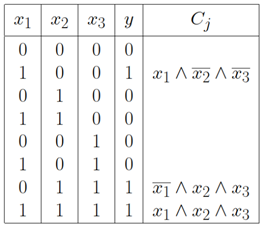
\includegraphics[scale=1.0]{images/arb_bool_funcs.png}
    \centering
    \caption{Table of values}
\end{figure}

What we can do is to build a network of TLUs that allow me to compute each of the component
for which the output has to be $1$ and then with a conjunction unit I put together all
the possible value with a or for merging the individual TLUs.

\begin{figure}[H]
    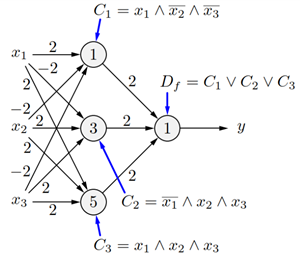
\includegraphics[scale=1]{images/arb_bool_funcs_graph.png}
    \centering
    \caption{Network of TLUs solving the boolean function}
\end{figure}


\subsection{Training TLUs}
The geometric interpretation that we have seen before about the operation of TLUs gives us the
understanding of how we can place the various parameters for our networks in order to
construct TLUs with $2$ and $3$ inputs.

But this makes sense when we are using $2$ or $3$ input, but this is something that is not
feasible when we are having more than three inputs, also this is not an automated method.

We want an automatic method for visualizing the space and points in the space, especially when
we have more then $3$ inputs.

What we want to do is to have an automatic way which adjusts the weights and the threshold
of the network so that I can reach the desired solution (if the two sets are linearly separable).

The \textbf{automatic training} of TLUs consist in the fact that we can start from a random value
of the weights and threshold, and then when we want to configure a TLU we need to evaluate
the error that we are generating at the output (of the TLU) in respect to the input pattern
that we have presented.

Basically, we have chosen randomly the threshold, the TLU generates an output, we evaluate
the error respect to the desired output, and then we try to adjust the weights and the
threshold to reduce the error.

We repeat this operation for all inputs until the error is really reduced or vanished.
\begin{enumerate}
    \item Start with random values for weights and threshold.
    \item Determine the error from the output of the TLU.
    \item Consider the error as a function of the weights and the threshold $e=e(w_1,...,w_n,\theta)$.
    \item Adapt weights and threshold so that the error becomes smaller.
    \item Iterate adaptation until the error vanishes.
\end{enumerate}

\subsubsection{Negation example}
\begin{figure}[H]
    \centering
    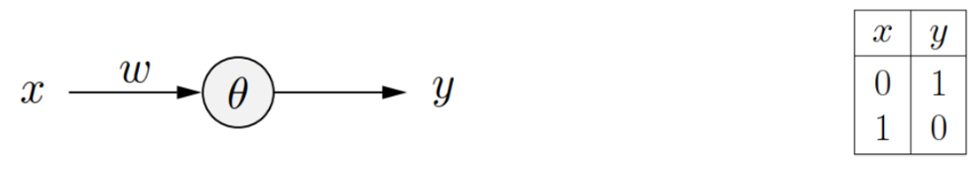
\includegraphics[scale=1]{images/neg_example.png}
    \caption{TLU that perform negation}
    \label{fig:neg_example}
\end{figure}
$$\neg x$$
In this case we have two really simple parameters, the weights and the threshold.
Let’s represent the error for all possible weights and all possible threshold at least
for a subset that we are interested in analyzing. Let’s consider the $x=0$, in this case
the desired output is $1$, if we take $w=2$ and we multiply it by $0$ the weighted input
will be $0$.

\begin{figure}[H]
    \centering
    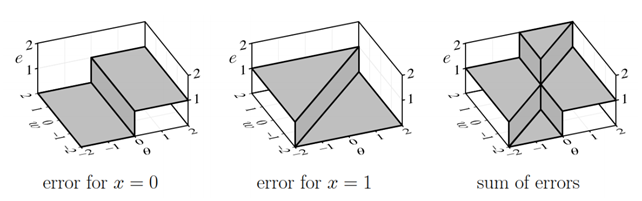
\includegraphics[scale=0.7]{images/errors_exampl.png}
    \caption{Diagrams of the errors expressed in terms of $\theta$ and $w$}
    \label{fig:neg_tlu_errors}
\end{figure}
Let's consider the first diagram on the left, with the various values of $\theta$ and $w$, and
with an input value of $x=0$.
Let's see the error that we have with the various possible combinations, we see that
for any values of the weight where the threshold is \textit{less} than zero, the \textbf{error}
is zero. Viceversa, for any value of the weight for a $\theta$ greater or equal to zero, the
error is one (a \textit{plateau}).

Now let's consider $x=1$, we are on the central diagram, in the left triangular part
of the domain there will be the error of $1$ defined $\forall w$.

Let's try to sum the errors and see what we obtains: we get an intersection for the error
equal to one, and also an intersection for the error equal to \textit{two} (which is strange,
since the error in this kind of example is always $1$ since the $y$ output is binary, but there
we are talking about a sum).

The only part where the error is equal to zero is a small triangle on the bottom. The problem
with this definition of the error is that is not suited for define an algorithm which allow
me to find the zero error.

\begin{figure}[H]
    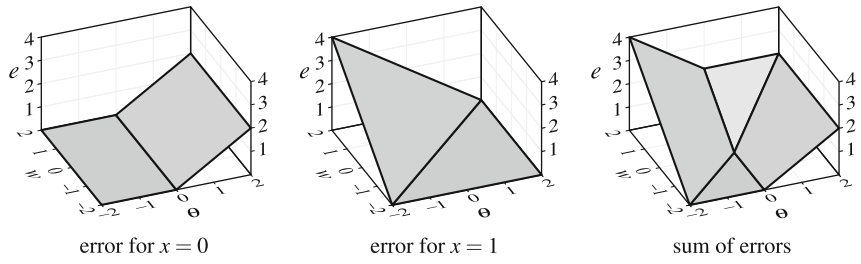
\includegraphics[scale=0.5]{images/desc_2_of_error.png}
    \centering
    \caption{Output error modified as function of weight and threshold}
\end{figure}

What i can do is modify the description of the error and consider that for each value
of the input i will not have just the error which is $1,0$ or $2$, but i will consider
a covering and continuos \textbf{surface area} (such that is possible to increase progressively
the error).

\begin{figure}[H]
    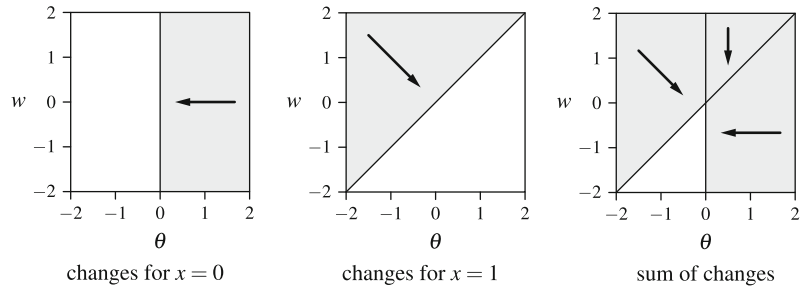
\includegraphics[scale=0.6]{images/desc_2_of_error_topview.png}
    \centering
    \caption{Top view output error modified as function of weight and threshold}
\end{figure}

So i can start from a random point and iteratively adapt parameters according to the direction
corresponding to the current point, i will stop if the error vanishes.

There are two ways of training a neural network:
\begin{itemize}
    \item \textbf{online learning}, we receive the learning pattern at time from the
          external environment, we compute the parameter corrections for this learning pattern (like
          we saw in the negation example) and in the end we apply the parameter corrections. In
          case of the \textit{negation}, first we adapt the weight and the threshold according to the left diagram,
          then we adapt them according to the middle diagram, then we adapt them again
          according to the left diagram and so forth until the error vanishes.

    \item \textbf{batch learning}, consists in not applying the changes immediately after every
          training example, but aggregating them over all training examples. Only at the end of
          a (learning/training) epoch, that is, after all training examples have been traversed,
          the aggregated changes are applied. Then the training examples are traversed again
          and at the end the weight and the threshold are adapted and so forth until the error
          vanishes.
\end{itemize}

\subsubsection{Delta rule (Widrow-Hoff)}
Given:
\begin{itemize}
    \item $\vec{x}=(x_1,...,x_n)^T$ be an input vector of TLUs.
    \item $o$ is the desired output for this input vector.
    \item $y$ the actual output of the TLU.
    \item $\eta$ as learning rate.
\end{itemize}
If $y\neq o$, then, in order to reduce the error, the threshold $\theta$ and the weight
vector $\vec{w}=(w_1,...,w_n)$ are adapted as follow:
$$\theta^{(new)}=\theta^{(old)}+\Delta\theta\text{, with }\Delta\theta=-\eta (o-y)$$
$$w_i^{(new)}=w_i^{(old)}+\Delta w_i\text{, with }\Delta w_i = \eta (o-y)x_i$$
$$\forall i \in \{1,...,n\}$$

The first equation is correction (delta) of the threshold and the second is the correction of the
weight. The variation is given by an expression which is proportional to the difference
between the actual and expected output (which is the error).

The correction for the weight is proportional not only to the error but also to the input.
Essentially, if i have an actual output smaller then the desired one, i take the input
that are bigger, and i try to push them to contribute more to the excitation
of \textit{threshold logic function} so that the output will be higher and as
consequence the error will be lower.

The $\eta$ controls the speed of updates, the bigger is the bigger will be the update.
\begin{figure}[H]
    \centering
    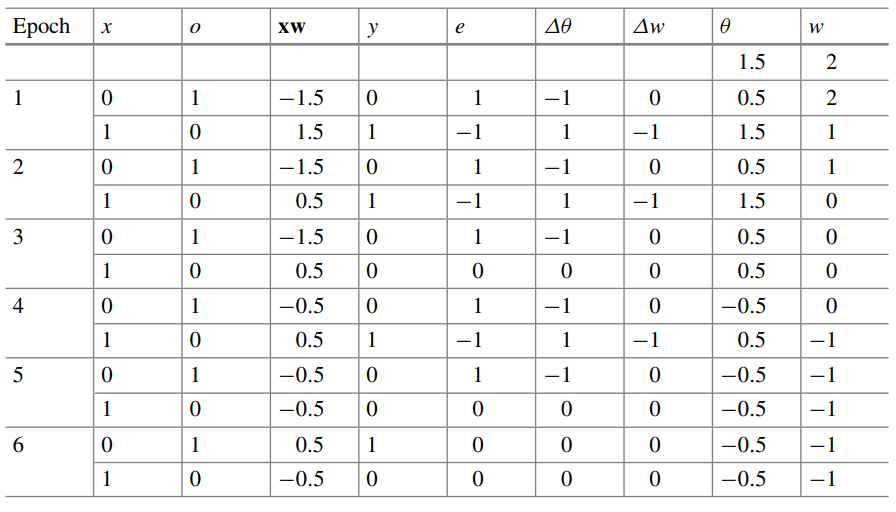
\includegraphics[scale=0.5]{images/online_training.png}
    \caption{Online training with $\theta = \frac{3}{2},w=2,\eta =1$}
\end{figure}

\begin{figure}[H]
    \centering
    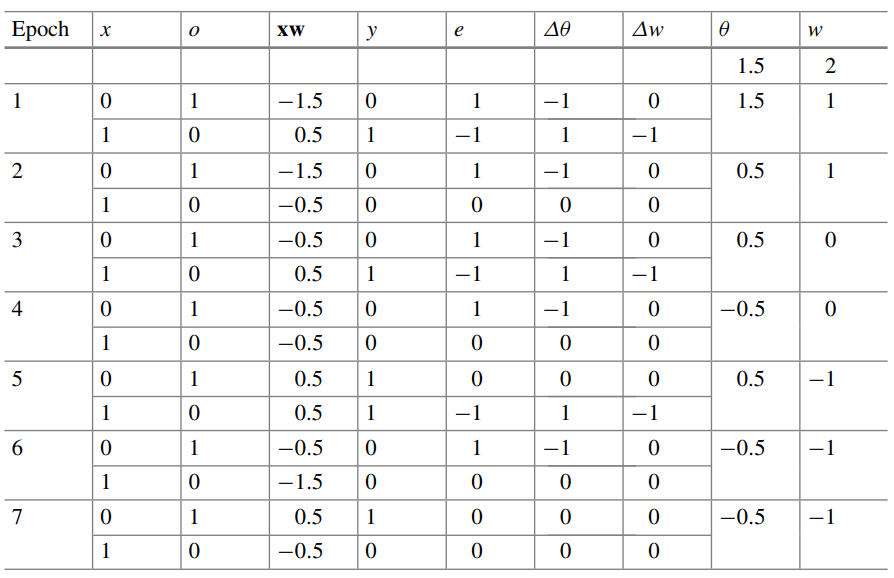
\includegraphics[scale=0.5]{images/batch_training.png}
    \caption{Batch training with $\theta = \frac{3}{2},w=2,\eta = 1$}
\end{figure}

Basically what happens in the online training, if i start in the first move i may go here,
and so on, i'll move one step at the time since the amount of change is control by the
learning rate.

in this case i move in one direction, since i apply together the two errors correction,
so i'm moving in combination of the two changes of the secondo batch, then again i'm applying
the two changes and i move. I do less move respect to the other since  i combine the two
correction for the expression that i shown.

I can try to do the same for the more complex case of the TLU, with two inputs. here i have
the conjunction with the truth table describing the implementation. What i'm doing basically
i have found the straight line that gives the satisfied and unsatisfied area for determining
the solution.

\subsubsection{Convergence theorem}
If we consider a set of training patterns: $L=\{(\vec{x},o_1),...,(\vec{x}_m,o_m)\}$,
each consisting of an input vector $\vec{x_i}\in\mathbb{R}$ and a desired
output $o_i\in\{0,1\}$.

Furthermore, let's consider $L_0=\{(\vec{x},o)\in L|o=0\}$ and
$L_1=\{(\vec{x},o)\in L | o=1\}$. If i can show that $L_0$ and $L_1$ are
\textbf{linearly separable}, then is possible to prove that we have a
$\vec{w}\in\mathbb{R}^n$ and $\theta\in\mathbb{R}$ such that:
$$\forall (\vec{x},0)\in L_0 :\vec{w}^T\vec{x} <\theta$$
$$\text{and}$$
$$\forall (\vec{x},1)\in L_0:\vec{w}^T\vec{x}\geq\theta$$

This means that is possible to divide the two sets, and then the online or batch
training procedure is able to terminate. So if the two sets are linearly separable they
will give us a final value in a \textbf{finite time}. The final error will e zero.

The problem is that if we are not able to perform the linear separation of $L_0$ and $L_1$,
the algorithm is \textbf{not able to terminate}. The algorithm will oscillate around and we
will not be able to find a solution with the zero error.

\begin{figure}[H]
    \centering
    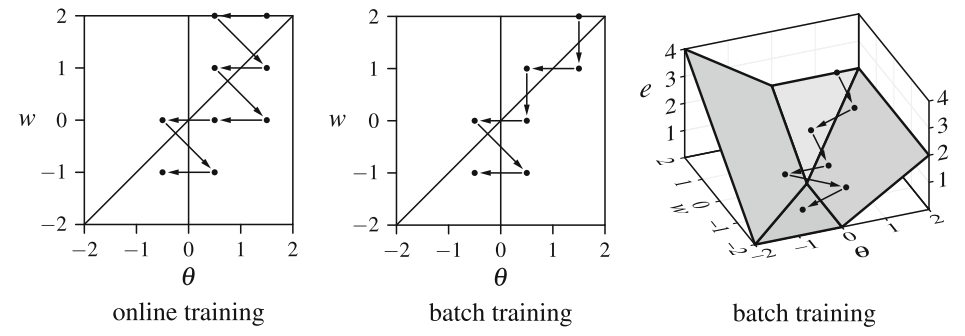
\includegraphics[scale=0.4]{images/batch_training_example_graph.png}
    \caption{Example of online and batch training (also with summed errors)}
\end{figure}

The correction of the parameters maybe slowed down due to the fact that we have $0$ and $1$
to the possible values for our outputs. This implies that if we have an output for our
threshold logic function equal to $1$, we can find an adjustment and apply it.
If we have an input which is $0$ whichever weight we have, we may not be able to compute
a correction that in the end will reduce the final error.

So when we apply an input which is one we can change the weight for finding a better value
for the configuration, if we apply the change on an input which is zero the possible changes
actually vanishes since we are multiplying by zero, we are not observing a variation.

To avoid to waste to much time on this issue, we can change the representation of the values,
for \textit{true} we are considering $1$ and for \textit{false} we are considering $-1$.

What we can point out, is that a \textit{single} TLU, is able to point out any linearly
separable function. We have just to apply the delta rule which is easy and fast and
guarantee to find a solution, if one exists.

The problem is given by a more complex structure, like a network of TLUs,
in this case we cannot apply directly the delta rule, because we have no clue
about which is the output. We need something more complex for managing that.

\subsection{Artificial neural network}
An ANN in general ha a very simple definition since it is a \textbf{directed}
graph $G=(U,C)$ composed by nodes and edges, in the graph we have processing
nodes that can elaborate the information incoming in, some arcs that
are bringing in the network some external information, and others that extract
the computation performed by our network (which is a structure that mimic our
brain).

The connections are the axon-synaptic connections which connect the nucleus of the
neurons. In a general neural network this is the very abstract definition, in practice
in order to use this kind of structure we will need to have more regular more focused
organization of neurons connections.

The set of vertices $U$ is partitioned into:
\begin{itemize}
    \item $U_{in}$ is the set of input neurons.
    \item $U_{out}$ is the set of output neurons, whi are the one delivering the
          result of the computation to the outside world.
    \item $U_{hidden}$ is the set of hidden neurons, they don't have any direct
          connection to the external world.
\end{itemize}

\subsection{General structure of the neuron}

\begin{figure}[H]
    \centering
    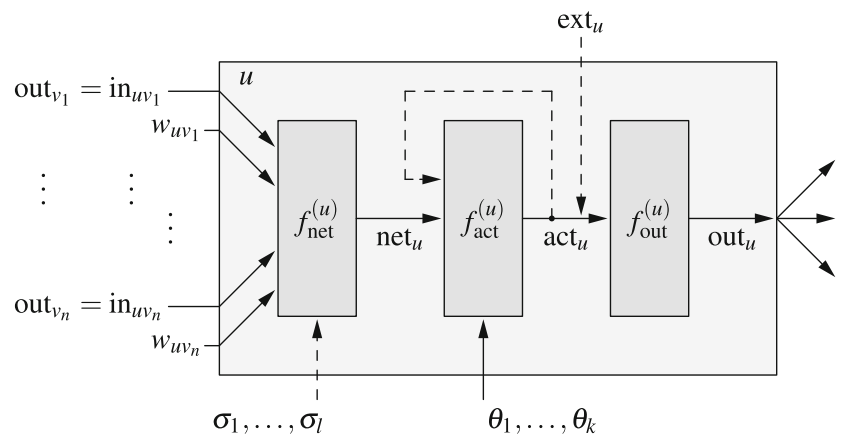
\includegraphics[scale=0.5]{images/general_structure_neuron.png}
    \caption{Internal representation of a neuron}
\end{figure}

We see that we have inputs that are coming in the network and usually this inputs are
manipulated in order to understand which is the global stimulus that the neuron
receive from the external world.

If an incoming signal from a previous neuron has relevance, we want to multiply the
amount o signal incoming in by an appropriate constant in order to have a stronger weight
for a subsequent processing in this neuron.

In this example we associate the weight $w_{uv_1}$, which is the weight for the neuron
$u$ respect to the incoming neuron $v_1$.

These inputs are processed by three stages in which we perform specific operations, we want
to see how much the neuron is actually solicited. For these reason we have three
stage functions:

\begin{itemize}
    \item The $f_{net}^{(u)}$, takes the input with the \textit{relative relevance} of the
          various inputs to generate the \textbf{global solicitation} for our neuron. This is a general
          definition, a specific definition changes in base of the network we are considering.

    \item The $f_{act}^{(u)}$, the activation functions analyze the network input from the
          previous function and generate the \textbf{excitation status} of our neuron. This will tell
          us if the neuron is sufficiently excited.

    \item The $f_{out}^{(u)}$, which takes the excitation status of the neuron and elaborate
          the final status of the neuron to deliver to the subsequent neurons.
\end{itemize}

In general we have also an external variable $ext_u$ which tell us how much the excitation
should be increased from a stimulus coming directly from the \textit{external world}
(not from previous neuron, from the external world).

These are the various inputs that any neuron can have, we may have both the input coming
from other neurons and the input coming from the external world, or we can have for a subset
of neurons only the stimulus coming from the external world and no other inputs.

We have input neurons coming which are weighted properly, these values are used
with the \textit{network input function} which is generating the global excitation status
coming from the other neurons, this one is will generate the \textit{activation status} of the neuron (how much it is
stimulated by the external neurons).

In the end we have the out function which evaluates the final status of the neuron, which
is delivered to the other connected neuron.

\subsection{Type of artificial neural network}
In the practice we won't use the general structure introduced before, we will have
different type of ANN:

\begin{itemize}
    \item \textbf{feed forward network} are ANN that doesn't contains any cycles, the
          acronym is FNN.
    \item \textbf{recurrent network} are ANN that contains cycles (backward connections),
          the acronym is RNN.
\end{itemize}

\noindent
The operation of a general ANN:
\begin{enumerate}
    \item \textbf{input phase}, where the external input are acquired by
          input neurons in the network.

    \item \textbf{work phase}, the external input are disconnect (by freezing
          the input neurons), we move the excitation generated by the input neurons
          to the connected neurons, we generate the stimuli for the connected neuron,
          we compute the output status of them and propagate the output to the
          neurons which are connected to this one.
\end{enumerate}

During the \textit{working phase} if the input of neurons are steady (input stimuli
are not changing), the computation of that neuron doesn't change (every stage
function generate the same values, FNN).

This is not the case when we have a RNN, since if one of the outputs connected to
a neuron is connected to an input will repeat the computation and this maybe change
the output status (due to \textit{recomputation}). I always say \textit{"may"}
since the actual change will depend specifically by the function that i'm using.
The \textbf{recomputation} of a neuron output occurs if any of its input changes,
we can't loop forever and not evolving. This means that the working phase continues
until the external outputs are steady, or a maximum number of
recomputation iterations is reached. The \textbf{temporal order} of computation
depends by the specific NN.
\newline
\newline
\noindent\textbf{Feed-forward neural network}
\begin{enumerate}
    \item Computation proceeds from input neurons progressively toward output neurons by following
          the topological order of the neuron in the network.
    \item The external inputs are frozen.
    \item Input neuron compute their outputs which are maintained steady and forwarded
          to the connected neurons.
    \item Neurons connected to preceding neurons with steady outputs generate their
          respective outputs and propagated forward to the subsequent neurons, until the
          external outputs are generated.
\end{enumerate}
\noindent\textbf{Recurrent neural network}
\begin{figure}[H]
    \centering
    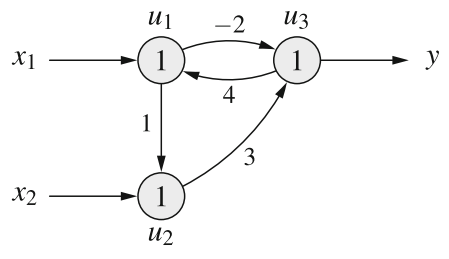
\includegraphics[scale=0.5]{images/RNN.png}
    \caption{A simple recurrent neural network}
\end{figure}
In the neurons there is the threshold which is considered for the operation,
and we have some interconnection weights which define the weights to be applied to the output
of a neuron when his output is delivered as input to a subsequent neuron.
\begin{figure}[H]
    \centering
    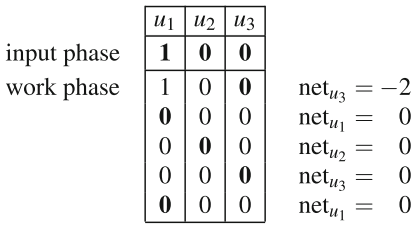
\includegraphics[scale=0.6]{images/RNN_simpl_ex1.png}
    \caption{Dataset for the previous RNN, for the $u_3,u_2,u_1$ order}
\end{figure}
In this case we choice to start from the input $1,0,0$ and with an updating order of
neurons that is $u_3,u_1,u_2,u_3,u_1,u_2,u_3,...$. Each bold number in working phase
entry of the table is an output of the \textit{ordered} neuron ($0$ if greater less than $\theta$
or viceversa $1$). In this case we can reach a steady state, and exit the RNN.
\begin{figure}[H]
    \centering
    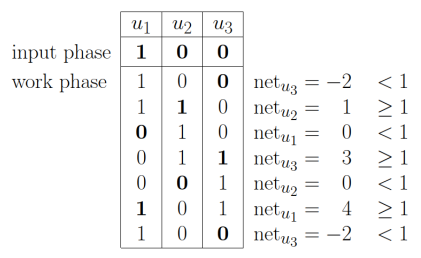
\includegraphics[scale=0.6]{images/RNN_simpl_ex2.png}
    \caption{Different dataset of the same RNN with $u_3,u_2,u_1$ order}
\end{figure}
Now let's consider a different ordering $u_3,u_2,u_1,u_3,u_2,u_1,u_3,...$, in this case
it is not possible to reach a steady state inside the RNN (\textbf{no stable state}, \textit{
    oscillation} of output).

\subsection{Configuration of a neural network}
The details of the configuration strictly depends from the
structure opf the network, in general we have two categories of
learning procedure (or training procedure):

\begin{itemize}
    \item \textbf{fixed learning task}.
    \item \textbf{free learning task}
\end{itemize}
\pagebreak
\noindent\textbf{Fixed learning task}
\newline
\noindent Considering a NN of $n$ input neurons $U_{in}=\{u_1,...,u_n\}$ and $m$ output neurons
$U_{out}=\{v_1,...,v_m\}$. A fixed learning task is a set of training patterns
$l=(\vec{i^{(l)}}, \vec{o^{(l)}})$, each consisting of:
\begin{itemize}
    \item an input vector $\vec{i^{(l)}} =(ext_{u_1}^{(l)},...,ext_{u_n}^{(l)})$
    \item an output vector $\vec{o^{(l)}} =(o_{v_1}^{(l)},...,o_{v_m}^{(l)})$.
\end{itemize}
\noindent At the end of the configuration the network is able to generate the desired output
that correspond to the output vector. Since the examples are composed by an input
vector and the expected output that we want to get, this is called \textbf{supervised
    learning}.

A fixed learning task is solved when for all training patterns $l\in L_{fixed}$ the
neural network computes, from the external inputs contained in the input vector
$\vec{i^{(l)}}$ of a training pattern $l$, the outputs contained in the
corresponding output vector $\vec{o^{(l)}}$.
\newline
\newline
\noindent\textbf{The error of a fixed learning task}
\newline
The error says how well a neural network solves a given fixed learning task. Essentially
it is the difference between desired and actual outputs.
$$e=\sum_{l\in L_{fixed}}e^{(l)}=\sum_{v\in U_{out}}e_v=\sum_{l\in L_{fixed}} \sum_{v\in U_{out}}e_v^{(l)}$$
$$e_v^{(l)}=\left(o_v^{(l)}-out_v^{(l)}\right)^2$$
In order to have a number which tell us the final quality what we need to do we have
to consider the module of the error, what we are doing is consider the difference between
the actual and the desired output. But in this simple difference could give us a final
number which is not reflecting the total accuracy of the NN due to the \text{sign}.

A solution to this is to use a squared value, in this way we can avoid the negative
sign.
\newline\newline\noindent\textbf{Free learning task}\newline
A free learning task is the complementary approach of the fixed learning task, in
which the desired behavior is not defined a priori by the pair of vectors for
the input and the output.

$$n\text{ input neurons }U_{in}=\{u_1,...,u_n\}$$
$$\text{one input vector }\vec{i^{(l)}} = \left( ext_{u_1}^{(l)},...,ext_{u_1}^{(l)}\right)$$

We only have a set of input vectors which are presented to the network and the
learning algorithm will lead to an output vector which is similar to the given input.

\noindent\newline\textbf{Preprocessing}\newline
In order to be sure that the learning is working properly, we have to be sure
that one of the input is dominating the operation of the network, as consequence
we have to do some preprocessing on the data in order to give the same relevance
to all neurons.

For each component of the input vector we need to compress the representation
in the same range, this is called \textbf{normalization} (according to the
average of the input value for each component, we need to be sure that
the variance $\sigma_k$ is normalized as well).
$$\mu_k =\frac{1}{|L|}\sum_{l\in L}ext_{u_k}^{(l)}$$
$$\sigma_k =\sqrt{\frac{1}{|L|-1}\sum_{i\in L}\left(ext_{u_k}^{(l)}-\mu_k\right)^2}$$

This is the standard normalization of the deviation $\sigma_k$, we have also another
possibility which is called \textbf{unbiased standard deviation} (often preferred
by statistician since is not polarized on the two direction).

If we apply the normalization this is the external stimuli that we will have after
the normalization, basically all the stimuli are recomputed with respect to the
average value and they are normalized in dimension dividing them by the standard
deviation.
$$\sigma_{u_k}^{(l)(new)}=\frac{ext_{u_k}^{(l)(old)}-\mu_k}{\sigma_k}$$

There is a problem that we have to seriously consider when we are looking
to our examples, we need to have \textit{sufficiently descriptive examples},
which have to be well distributed over the domain that i'm considering (not
focussing only on a portion of the domain).

So far we have been dealing with integer and real numbers, we want to use
symbols for represent a group of examples that are similar together in a concise way.

For doing that we need to associate a group of identifiers to a group of examples. For
being able to represent this symbols we consider the \textbf{1-in-N encoding}, if
we need to represent $n$ symbols we have a string of $0$ and $1$ and only one bit the one
that corresponds to the symbol we want to represent will be $1$ (the others will be $0$).

\subsection{Multi-layer Perceptrons}
A \textbf{multi-layer perceptrons} it is essentially a feed-forward neural network
in which is present a strictly layered structure. They neurons are connected in groups,
each groups receives the input only from the previous layer or from the external input.
The output is delivered by the subsequent group, there are different kinds of layers:

\begin{figure}[H]
    \centering
    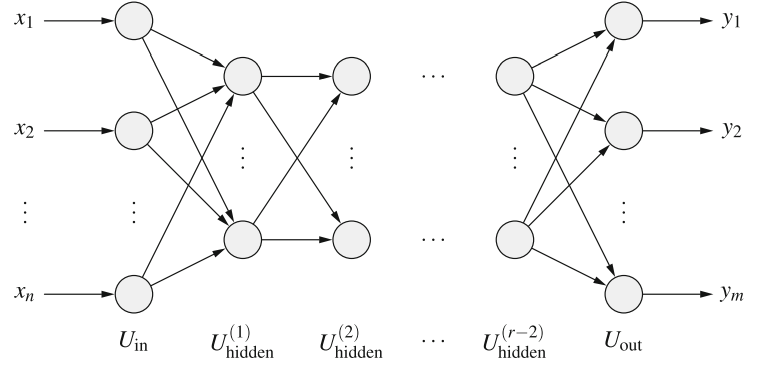
\includegraphics[scale=0.5]{images/multi-layer-percep.png}
    \caption{General structure of $r$-layered perceptron}
\end{figure}

\begin{itemize}
    \item \textbf{input layer}
    \item \textbf{hidden layer}
    \item \textbf{output layer}
\end{itemize}

Each layers is connected, in multi-layer perceptrons the neurons are strictly connected
between layers, jump are not allowed (like in the feed-forward network).

The network input function of each \textit{hidden neuron} and of each \textit{output neuron}
is the \textbf{weighted sum} of its inputs:
$$f_{net}^{(u)}(\vec{w_u},\vec{in_u})=\vec{w_u}\vec{in_u}=\sum_{v\in pred(u)}w_{uv}out_v$$

The activation function of each hidden neuron is a so-called \textbf{sigmoid function},
that is, a monotonically non-decreasing function with:
$$f:\mathbb{R}\rightarrow [0,1]\text{ with }\lim_{x\rightarrow -\infty}f(x)=0\text{ and }\lim_{x\rightarrow\infty}f(x)=1$$

It has a shape that allows a minimum and a maximum value (shaped), such that the possible \textit{net status}
of the neurons are inside the continuos domain between $0$ and $1$ of the function (squishification of the net status).
If i have enough excitation in the network status the sigmoid function will give a positive excitation of the neuron,
viceversa, it will point out a lower value in the function.
\begin{figure}[H]
    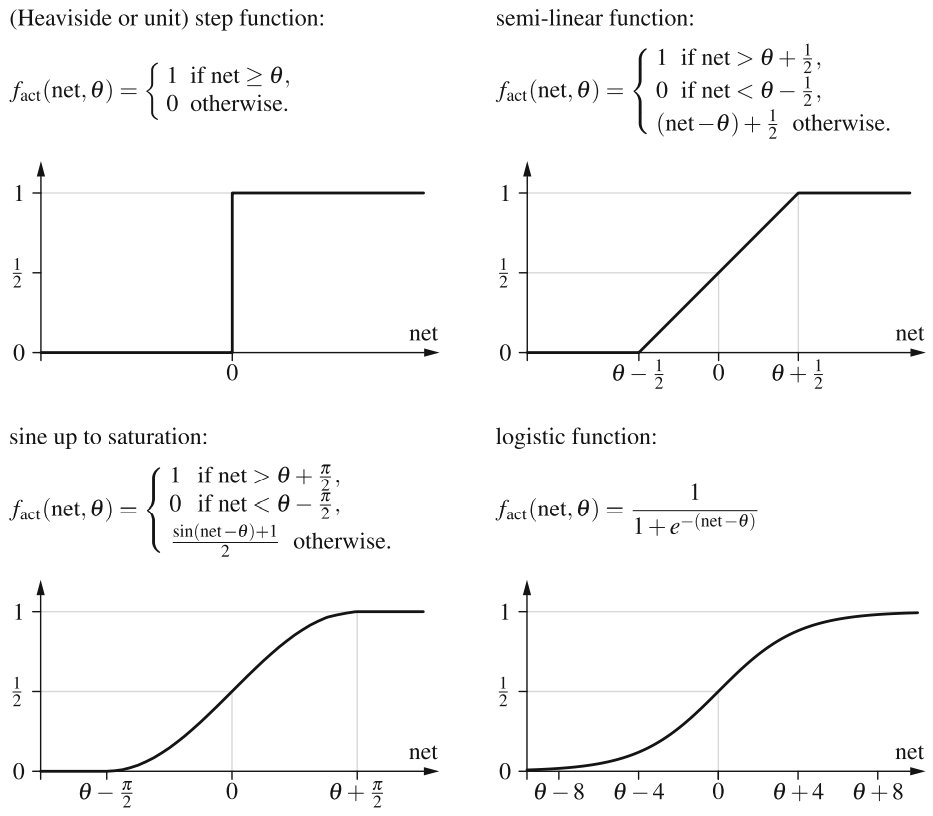
\includegraphics[scale=0.45]{images/sigmoid_functions.png}
    \centering
    \caption{Some \textbf{unipolar} sigmoid activation functions}
\end{figure}
In the contemporary NN the sigmoid function are rarely used, actually the \textbf{ReLU} (\textit{Rectified Linear Unit})
function is much more used since it is much easier to train (more similar to the behavior of the biological neurons).
\begin{figure}[H]
    \centering
    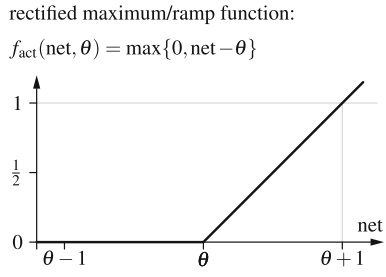
\includegraphics[scale=0.5]{images/relu.png}
    \caption{ReLU function}
\end{figure}


The activation function of each output neuron can be a sigmoid or can be a \textbf{linear}
function (depends on what we want to achieve). There are many types of sigmoid function for representing
the general behavior, the most simple is the \textbf{step function}.

I have a $0$ value until my network excitation reach the value $\theta$, then the output
of excitation jump to the strongest status (the value of minimum and maximum activation are
generally $0$ and $1$).

If you prefer a smoother approach you can use the $sin$ approach were the derivative
is progressively approaching the maximum value.

A \textbf{logistic} function is a function with the same shape but that doesn't reach a saturation
at the extremes of the range. In this way it is possible to consider the inverse
of the function, otherwise it is not possible.

We may have some problems during the learning operation when using the \textit{step function},
since when we have $0$ we won't have any effect on the output of the neuron,
even if we change the activation the output will be $0$. As solution it is possible to
use \textbf{bipolar} (opposite to the unipolar, which extends only in one pole)
sigmoid functions, which changes the ranging to $[-1,+1]$, like the \textit{hyperbolic tangent}.

\begin{figure}[H]
    \centering
    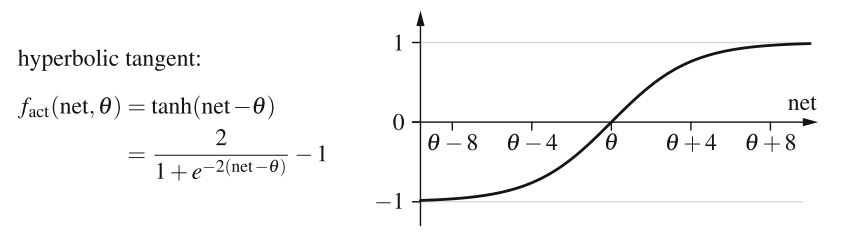
\includegraphics[scale=0.5]{images/hyperbolic_function.png}
    \caption{Bipolar sigmoid activation function (\textit{hyperbolic tangent})}
\end{figure}

I can describe the group of connections between two \textit{consecutive} layers of
a multi-layer perception by using a $n\times m$ matrix. Which is the collection of the
connection weights between the layers:

\begin{figure}[H]
    \centering
    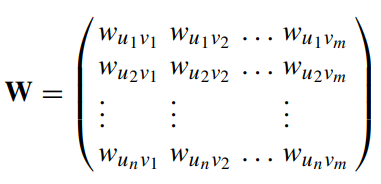
\includegraphics[scale=0.5]{images/weight_matrix.png}
    \caption{Matrix describing connection weights between two layers}
\end{figure}

As a consequence the computation can be described in a very simple way,
by using the vectors:
$$\vec{net_{U_2}}=\textbf{W}\vec{in_{U_2}}=\textbf{W}\vec{out_{U_1}}$$
You just take the vector of the input neurons of the second layer
(which are the output of the preceding layer) and multiply by the
weight in between the layers.

Then you apply the sigmoid function $\sigma$ for squish the values between $[0,1]$,
you can also use a \textbf{bias} value for each independent values by using a vector $\vec{b}$.
The bias tells you \textit{how high} the threshold has to be in order for the neuron to fire.
$$\sigma\left(\textbf{W}\vec{in_{(U_2)}}+\vec{b}\right)$$
Let's consider an example with the \textbf{bi-implication}
three-layer perceptron:

\begin{figure}[H]
    \centering
    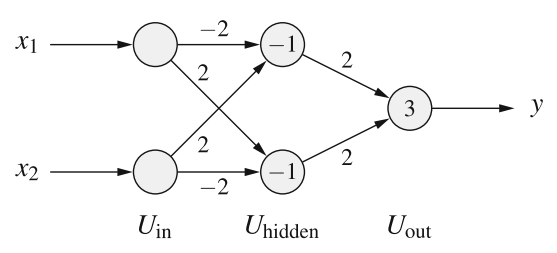
\includegraphics[scale=0.5]{images/three_layer_example.png}
    \caption{Three-layer perceptron for bi-implication}
\end{figure}

\begin{figure}[H]
    \centering
    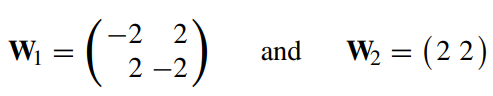
\includegraphics[scale=0.5]{images/weights_three_layer_example.png}
    \caption{Weight matrices for the input and hidden layers}
\end{figure}

The only difference respect the TLUs network of bi-implication is that
each neuron can be an input,hidden and output neuron. In this configuration
we are dividing everything in layer of neurons, so we have to \textbf{add} a
input layer for that (in respect to using TLU).

So far we have seen boolean function, but what we want to look now is how we can extend
the dimensions of a feed-forward network in order to consider not only
the boolean function of the TLUs but we want to consider in a multi-layer
perceptron any type of real number (extend the capability of describing the world).

We can see that the multi-layer perceptron,
with any input real-number can be used for function approximation.
\newline\newline\noindent\textbf{Function approximation}\newline
Consider the function in the diagram, it is very simple and continuos,
and let's consider the points $x_1,...,x_4$ where we want to compute
the value of the function and we want to find a method to approximate for any other value
$x$ a value in that function.

What i can do is to consider the \textbf{midpoint Riemann integration}.

\begin{figure}
    \centering
    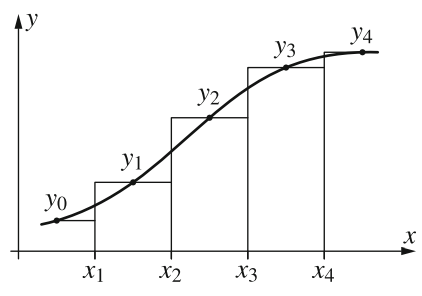
\includegraphics[scale=0.5]{images/midpoint_integra.png}
    \caption{Approximating a continuos function with step functions}
    \label{fig:midpoint_int}
\end{figure}

\begin{itemize}
    \item Approximate a given function by a step function.
    \item Construct a neural network that computes the step function.
    \item Error is measured as the area between the functions.
\end{itemize}

It is possible to prove that if you take any Riemann integrable function,
it can be approximated with arbitrary accuracy by a \textit{four-layer
    perceptron}.

\begin{figure}[H]
    \centering
    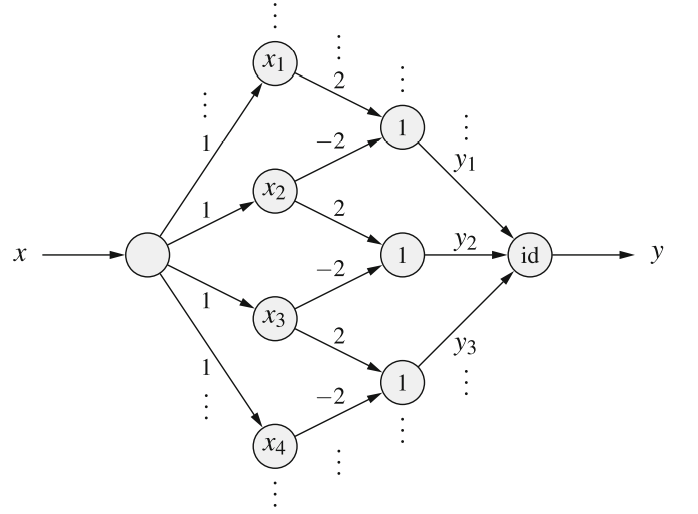
\includegraphics[scale=0.5]{images/integra_perceptron.png}
    \caption{NN that computes the step function for integration}
\end{figure}

The input $x$ is taken by an input neuron, then we have the first
layer composed by the subdivision of the domain in the points
$x_1, x_2, x_3,x_4$.

In the second hidden layer, we create one neuron for each step,
which receives input from the two neurons in the first hidden layer that
refer to the values $x_i$ and $x_{i+1}$ marking the border of the step.
Only one neuron in the second layer can be active, and it will represent
the step where the input values lies (this through the \textbf{combined
    excitation} of the neurons in the first hidden layer).

The connection from the neurons of the second layer to the output
neuron are weighted with the function values of the stair steps that
are represented by the neurons.

Since only one neuron can be active on the second hidden layer, the
output neuron receives as input the height of the stair step , in which
the input value lies, as result it computes the correct sampling
of the function saw in figure \ref{fig:midpoint_int}.

The multi-layer perceptrons can be considered an \textbf{universal
    approximators} of the Riemann integration technique, with the maximum
desired error (i can choose the maximum error i want to get for my
function by choosing the number of neurons for get that accuracy).\newline\newline
\noindent\textbf{Delta approximation approach}\newline\noindent
We can actually simplify the error by considering a trick instead of using the
combined excitation.

I can split the domain of the function for my network in parts like before,
then instead of defining the value of the function for each interval i just
use iteratively the $\Delta$ variation respect to the value considered.

\begin{figure}[H]
    \centering
    \caption{}
    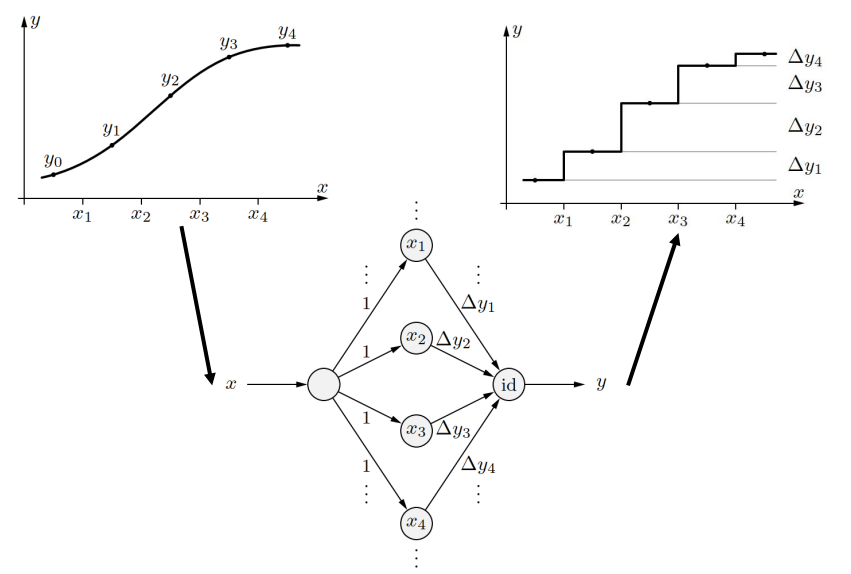
\includegraphics[scale=0.5]{images/multi-delta-integra.png}
    \label{fig:integra_delta}
\end{figure}

The structure of the network (figure \ref{fig:integra_delta}) will be simpler
because i will distribute the input of the hidden neurons,
that will tel me if the value $x$ is before $x_i$ or greater than $x_i$ (i don't care where).

For example, if the value is between $x_1$ and $x_2$ the first neuron
will generate $\Delta y_1$ and this will be delivered in output.

If i have a value between $x_2$ and $x_3$ i will still have $x_1$ that
will be excited enough and will generate the \textit{contribution}
for the output ($x_1$ and $x_2$ will be both excited, their
contribution will be summed up and then delivered to the output).

This will make simpler the structure of the network.

\subsection{Regression}
Let's find a way for approximate a function without using the basic calculus approach. In
order to do this we have to understand the concept of \textbf{regression}.
We saw that for training an ANN we need to minimize the error function, which is computed by
considering the squared difference between desired output and actual output.

The regression is a technique used in statistical analysis for extrapolating a straight
line that better approximate the existing relationship inside a dataset.

Formally, considering the dataset $G=\{(w_0,y_0),...,(w_n,y_n)\}$ let's imagine it exists a functional relationship
between the input vector $w_i$ and the abscissa $y$, then the regression will help us to find
the parameters of that function. Different kind of functions will give us different kind of regressions.

\subsubsection{Linear regression}
If we expect that our quantities $x$ and $y$ exhibits a linear dependence, then we have
to identify the parameters $a$ and $b$ that extrapolate the straight line $y=g(x)=a+bx$.
In general, won't be possible to find a straight line that traverse all the points of the
dataset. What we will do is finding a straight line which deviates the lest possible,
so that minimize the error as follows:
$$F(a,b)=\sum_{i=1}^{n}(g(x_i)-y_i)^2=\sum_{i=1}^n(a+bx_i-y_i)^2$$

The necessary condition to find the minimum is given us by mathematical, if i take the
partial derivatives between the two parameters $a$ and $b$ (which are the variables
in the formula) setting this partial derivatives of th error to $0$ it will give to
me the condition that allow us to find the minimum (\textit{Fermat's theorem}).

$$\frac{dF}{da}=\sum_{i=1}^{n}2(a+bx_i-y_i)=0$$
$$\frac{dF}{db}=\sum_{i=1}^{n}2(a+bx_i-y_i)x_i=0$$

The \textit{linear algebra} tells me the solution is unique unless i'm so unlucky that
all the values $x$ coincides, in that case i have basically one equations but
two variable ($a$ and $b$) and as consequence infinite solutions.

For example, if i need to find the regression of these points:
\begin{figure}[H]
    \centering
    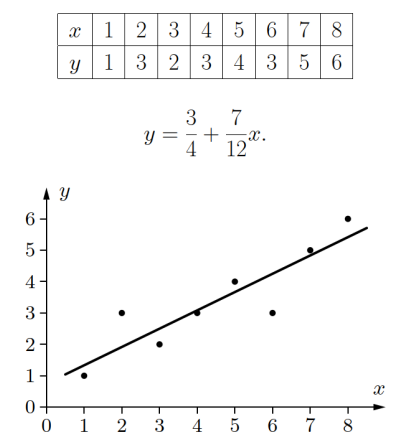
\includegraphics[scale=0.7]{images/regression_line.png}
    \caption{Regression line example}
    \label{fig:regression_line}
\end{figure}

\subsubsection{Polynomial regression}
The previous method is generalizable to polynomial of arbitrary order.
The model i have considered is not a good model, is too approximate, i can look if there
is instead a very simple straight line a polynomial.
Instead of considering a polynomial of grade one, i consider a polynomial of grade $m$.

$$y=p(x)=a_0+a_1x+...+a_m x^m$$

The minimization fo the error now can be generalized in this way:

$$F(a_1,...,a_n)=\sum (p(x_i)-y_i)^2=\sum(a_0+a_1x+...+a_n x^n-y_i)^2$$

Like in the linear regression, the necessary conditions for the function to be
minimized (finding the minimum), are that the partial derivatives respect to the
parameters $a_i$ vanishes:

$$\frac{dF}{da_0}=0,\frac{dF}{da_1}=0,...,\frac{dF}{da_m}=0$$

\begin{itemize}
    \item This system can be solved by using the standard methods from linear algebra.
    \item The solution is unique unless the points lie extactly on a polynomial of
          lower degree.
\end{itemize}

\subsubsection{Multilinear regression}
Until now i just tried to make the approximation more accurate going in the
direction of polynomial,\textit{what happens if i have a function in multiple variables?}
$$z=f(x,y)=a+bx+cy$$
If i want to do a multi-linear regression (since i'm applying linear regression to a function
of two variables), i have just to apply what i wast doing before.

I have to consider the error in the approximated function $f$, and the actual value given
by the samples $z_i$ that i'm collecting (minimizing the sum of squared errors):

$$F(a,b,c)=\sum_{i=1}^{n}$$

What we need to do? again we need to find when the error is going to $0$, this happens when
the partial derivatives of the parameters are $0$.

$$\frac{dF}{da}=\sum_{i=1}^n 2(a+bx_i+cy_i-z_i)=0$$
$$\frac{dF}{da}=\sum_{i=1}^n 2(a+bx_i+cy_i-z_i)x_i=0$$
$$\frac{dF}{da}=\sum_{i=1}^n 2(a+bx_i+cy_i-z_i)y_i=0$$

As already said multiple times, the linear algebra will allow me to solve
this problem since i have three parameters $a,b,c$ and three equations.

Except the unfortunate case where all points are on a straight line, because in this case
i have a plane that can be rotated in any direction and i have \textit{infinite solutions}.

I can consider trying to approximate with a multi-linear regression a function that
is defined on $m$ different variables, this is the generalization of what we have
seen previously (difficult to draw):

$$y=f(x_1,...,x_m)=a_0+\sum_{k=1}^{m} a_k x_k$$

I have to minimize the sum of squared errors (vectors for parameters and matrices to define
the various values):

$$F(\vec{a})=(\textbf{X}\vec{a}-\vec{y})^T(\textbf{X}\vec{a}-\vec{y})$$

where:
\begin{figure}[H]
    \centering
    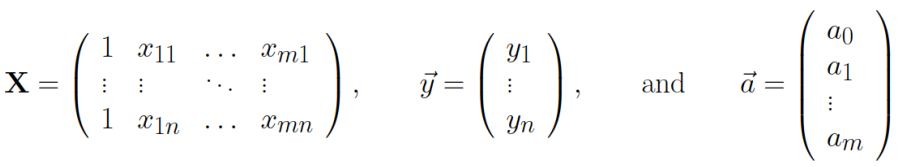
\includegraphics[scale=0.5]{images/parameters_multilinear_regre.png}
    \label{fig:infos_multilinear}
    \caption{Various $x$ values and vector parameters}
\end{figure}
I need to define the \textbf{gradient} which is the generalization of the previous definition
defined on vectors and not on the partial derivatives of functions as we seen before.
We need to look where the gradient is $0$ which will give us the \textit{hyperplane}
touching the surface in the minimum.
$$\vec{\nabla}_{\vec{a}} F(\vec{a})=\vec{\nabla}_{\vec{a}}(\textbf{X}\vec{a}-\vec{y})^T(\textbf{X}\vec{a}-\vec{y})=\vec{0}$$

This comes out as set of regular equations and linear algebra will allow us to solve it as
usual unless there is the singular case (if i have all points aligned to a single straight line
the plane which is minimizing my error is not defined).

The system of normal equations:
$$\textbf{X}^T\textbf{X}\vec{a}=\textbf{X}^T\vec{y}$$

which has solution unless $\textbf{X}^T\textbf{X}$ is a singular:

$$\vec{a}=(\textbf{X}^T\textbf{X})^{-1}\textbf{X}^T\vec{y}$$

\subsubsection{Logistic regression}
In the situation in which the dataset is not approximated with sufficient accuracy
from a polynomial function, we could use different kind of functions, for example:
$$y=ax^b$$
We can transform this in a linear equation by applying the operation of logarithm:
$$\ln{y}=\ln{a}+b\cdot\ln{x}$$
In the case of ANN we are interested in particular at the \textbf{logistic function}:
$$y=\frac{Y}{1 + e^{a+bx}}$$

If we apply the logarithm of this equation we can derive a different expression of our
function $y$ so that the description of this function will be a \textbf{linear description}.

Since lot of ANN uses as proper neuron activation function the logistic function,
if we would find a way for applying the regression method on that we could determine
the parameters of any network.

If we would find a way for applying the method of regression om the neurons, we could
determine the parameters of any network at two layers of only one point. The value $a$
of the function represent the threshold of the output neuron, while the value of $b$
represent the weight of the input. We can linearize the logistic function by applying
the following transformations (called \textbf{logit transformation}):

$$y=\frac{Y}{1+e^{a+bx}}\longleftrightarrow\frac{1}{y} = \frac{1+e^{a+bx}}{Y}
    \longleftrightarrow\frac{Y-y}{y}=e^{a+bx}\longleftrightarrow\ln{\left(\frac{Y-y}{y}\right)}=a+bx$$
\begin{figure}[H]
    \centering
    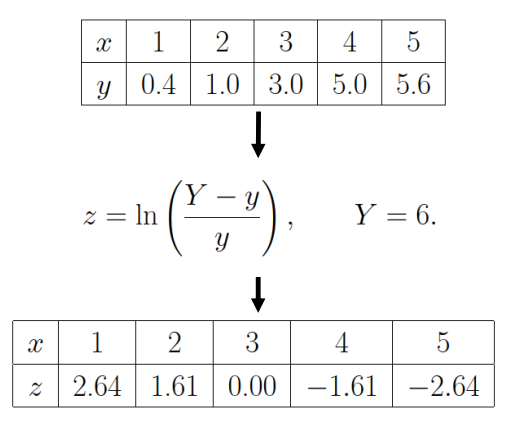
\includegraphics[scale=0.5]{images/logistic_regre_1.png}
    \label{fig:regr_1}
    \caption{Example of logistic regression}
\end{figure}
The results of the regression line in the example are:
$$z\approx -1.3775x+4.133, y\approx\frac{6}{1+e^{-1.3775x+4.133}}$$

\begin{figure}[H]
    \centering
    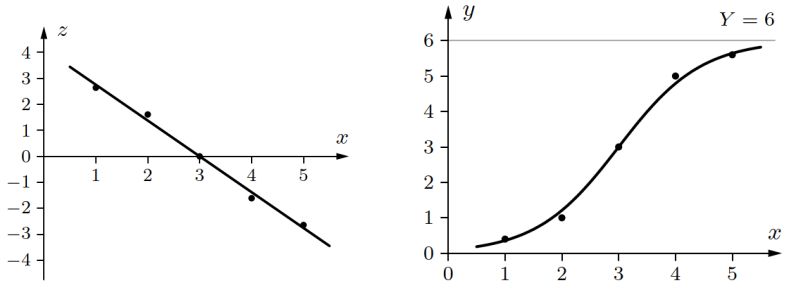
\includegraphics[scale=0.5]{images/regression_line_2.png}
    \label{fig_regr_2}
    \caption{Plot of logistic function}
\end{figure}

How can we understand the values of this non polynomial approximation by transforming it
applying the log transformation, so that we can perform the approximation on a
function that appear to be linear and then transform it back on the original function.

We can consider a logistic function defined on two variables, and we have this bi-dimensional
shape defined on two arguments. we can apply the same principle that we see before, this
can be used to solve a problem of separating two groups of examples of different classes (or
group).

$$y=\frac{1}{1+exp(4-x_1-x_2)}=\frac{1}{1+exp\left(4-(1,1)^T(x_1,x_2)\right)}$$
\begin{figure}[H]
    \centering
    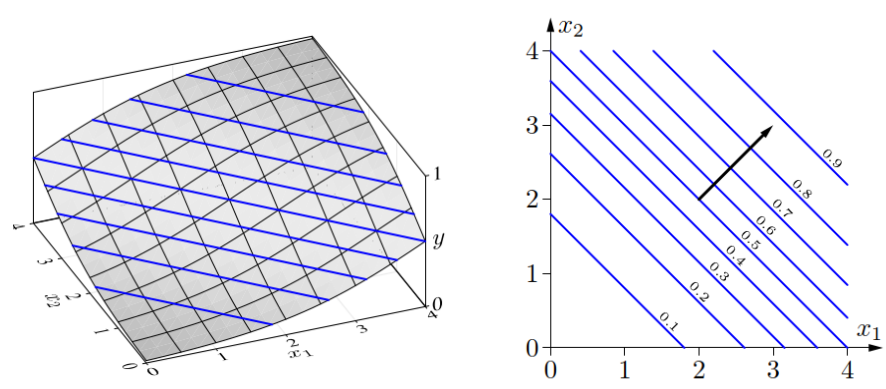
\includegraphics[scale=0.45]{images/logist_bidiminesional_reg.png}
    \caption{Plot of logistic function with two arguments}
\end{figure}

\subsubsection{Two-class problems}
Basically the two class problems can be solved by considering the two attributes,
which are the name of the class ($C$ is the class of attributes) and a vector random of $m$ dimension.
$$dom(C)={c_1,c_2}$$

We consider the \textbf{probability} of belonging to the first class $c_1$
and the probability to be in the second class $c_2$.

$$P(C=c_1|\vec{X}=\vec{x})=p(\vec{x})$$
$$P(C=c_2|\vec{X}=\vec{x})=1-p(\vec{x})$$

Given a dataset of points $X={\vec{x_1},...,\vec{x_n}}$, each of which belongs to one
of two classes $c_1$ and $c_2$.

Basically i want to get a \textbf{simple description of the function} $p(\vec{x})$, if i have
this function i can apply the \textbf{logistic description}:

$$p(\vec{x})=\frac{1}{1+e^{a_0+\vec{a}\vec{x}}}=\frac{1}{1+exp(a_0+\sum_{i=1}^m a_i x_i)}$$

Then i can apply the \textbf{logistic transformation} so that i can obtain the
\textbf{formal description} of the probability of being on one or the other class:

$$\ln{\left(\frac{1-p(\vec{x})}{p(\vec{x})}\right)}=a_0+\vec{a}\vec{x}=a_0+\sum_{i=1}^m a_i x_i$$


\textit{How can i find the specific value of the probability (and so solving the splitting of the
    example)?}
We can consider a specific function called \textbf{kernel} that describes
how strongly a data point influences the probability estimate for neighboring points.


which give us the correlation
in the examples, given some examples how can i say that the example that i observed
belongs to the group is influenced by similar examples, or belong to the other group
which means that is similar to the examples of the other group.

With a kernel we can describe the similarity of a
group of examples, the \textbf{Gaussian function} is commonly used. A function like this
tell me that if the picked data point is similar to the elements in the middle area, in that
case i have a significant value of the function, the more i go far from the values
which are similar the less is the value of the function.

$$K(\vec{x},\vec{y})=\frac{1}{(2\pi\sigma^2)}exp\left(-\frac{(\vec{x}-\vec{y})^T(\vec{x}-\vec{y})}{2\sigma^2}\right)$$


If i want to estimate the \textbf{probability density} i will use this expression:
$$\hat{f} (\vec{x}) = \frac{1}{n} \sum_{i=1}^n K(\vec{x},\vec{x}_i)$$
The kernel estimation applied to a two-class problems:
$$\hat{p}(\vec{x})=\frac{\sum_{i=1}^n c(\vec{x_i})K(\vec{x},\vec{x_i})}{\sum_{i=1}^n K(\vec{x},vec{x_i})}$$

If it is $$c(\vec{x})=1$$ the $x_i$ will belong to class $c_1$ if $c(\vec{x})=0$ otherwise.

\subsection{Training multi-layer perceptrons}
\subsubsection{Gradient descend}
\paragraph{3Blue1Brown}
Conceptually we think about each neuron to be connected to each neuron of the previous layer,
and the weighted sum of this neurons expresses the strength of this connections:
$$\sigma(w_1u_1+w_2u_2+...+w_nu_n+b)$$
If we consider all the weights and bias initialized randomly, the MLP network will perform
pretty terrible (he is acting randomly).

What you do is defining a \textbf{cost function} that can express if the result of the NN
is good or bad (for our objective). The greater the function is the greater is the error of the
NN respect to desired output.
$$e_v^{(l)}=\left(o_v^{(l)}-out_v^{(l)}\right)^2$$
So then what you do is considering the average cost function over all the samples inside the
NN, it is a cost value that express how good or bad the network is.

We want to use this error in such a way that we can perform better during the next execution,
let's consider a function $C(w)$ representing just one cost, if we want to find the input that
minimize the cost of this function we just have to take the derivative $\frac{dC}{dw}(w)=0$, but
this is not really feasible for complicate functions. You can find different \textbf{local minimum}
of the function, so what you find isn't the best possible cost function value that you will find.
Find the global minimum is pretty hard.

But our function will be much more complicated, since we are dealing with lot of parameters (like
the weights and the biases), let's imagine now a function with two variables where the cost
function is graphed as a surface above the $xy$ plane. Now, for minimizing the function i should
ask my self, in \textit{which direction the $C(x,y)$ function decreases most quickly?}, multi-variable
calculus has a concept of \textbf{gradient}, which is the direction of the steepest increase $\vec{\nabla} C(x,y)$,
and more to that the \textit{length} of that vector expresses how much steep is the increase.
The algorithm essentially will be:
\begin{itemize}
    \item Compute $\vec{\nabla}C$
    \item Small step in direction $-\vec{\nabla}C$
    \item Repeat until convergence
\end{itemize}

The negative gradient of the cost function will tell you how to change all the weights and biases
for all the connections, to efficiently decrease the cost (no overshot). The backpropagation
is an algorithm for computing that \textit{crazy} gradient.

The gradient is a vector expressed as $n$-dimension, where $n$ depends by weights and biases,
it is usually a giant number (impossible to visualize). The important thing, is that the
magnitude of each component (so the value) will tell you \textbf{how sensitive} the
cost function output will be respect to the weight and bias (how much it moves respect the previous
value).

\paragraph{Lesson notes}
Now we have to apply this for all the values for all the weights of the network. Essentially when
we talk about \textbf{training} or the process of learning of a NN it's just about minimizing the
cost function (or error function). More to that, the negative gradient vector will store
the relative importance of the weights for each neurons.

What we want to do is to follow the idea of the \textbf{gradient descent}, we want
to find the \textit{local minimum} of an error function in order to find the proper set of weights.

\begin{figure}[H]
    \centering
    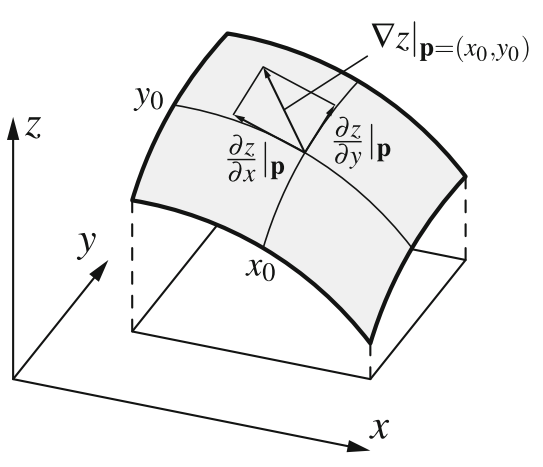
\includegraphics[scale=0.5]{images/gradienmt.png}
    \caption{Intuitive interpretation of the gradient of a real-valued function $z=f(x,y)$ at
        a point $(x_0,y_0)$}
    \label{fig:err_surface}
\end{figure}

Considering this error surface (figure \ref{fig:err_surface}), if we are in the
central point we can look to the derivatives of the error function in the two directions,
the \textbf{gradient} $\nabla$ is the vector tangent to the surface and will tell us the direction where
the surface is more or less increasing.

If we want to find the solution for our learning we need to look for the minimum of this
error function, so actually we need to look to the opposite direction to the gradient and we
look to reach the minimum.
$$e=\sum_{l\in L_{fixed}}e^{(l)} =\sum_{v\in U_{out}} e_v=\sum_{l\in L_{fixed}}\sum_{v\in U_{out}}e_v^{(l)}$$

So we need to evaluate the gradient to find the direction of the decreasing value, and
we need to go in the proper direction in order to reduce the error. In the case of the MLP
calculate the gradient means compute the partial derivative of the error function in respect
of the threshold and the weights taken as parameters.

Given $\vec{w}_u=(-\theta,w_{u_1},...,w_{u_k})$ as the vector of weights of a single layer
extended with the threshold, then compute the gradient as follow:
$$\vec{\nabla}_{\vec{w}u}e=\frac{\partial e}{\partial\vec{w}_u}=\left(-\frac{\partial e}{\partial\theta_u},\frac{\partial e}{\partial w_{up1}},...,\frac{\partial e}{\partial w_{up_n}}\right)$$

Since the total error $e$ is given by the sum of the individual errors in respect to all
neurons and all training patterns $l$, we get that:
$$\vec{\nabla}_{\vec{w}_u} e=\frac{\partial e}{\partial\vec{w}_u}\sum_{l\in L_{fixed}}e^{(l)}=\sum_{l\in L_{fixed}}\frac{\partial e^{(l)}}{\partial\vec{w}_u}$$

\begin{figure}[H]
    \centering
    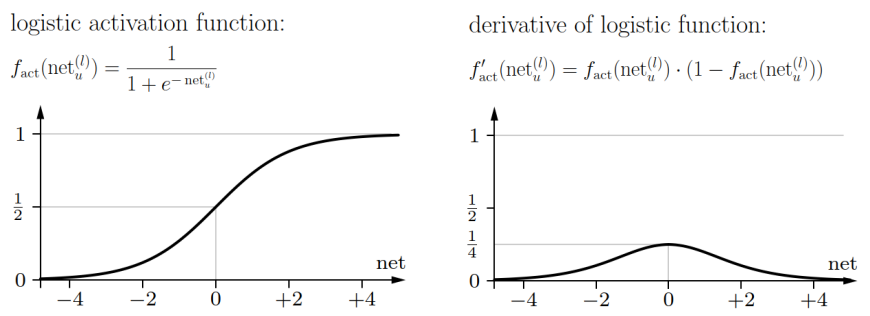
\includegraphics[scale=0.5]{images/logistic_gradient.png}
    \caption{Logistic function as activation function}
    \label{fig:log_func_gradient}
\end{figure}

If we have a \textbf{logistic function} as $f_{(act)}$ we will have that the changes
performed on the vector $\vec{w}_u$ will be proportional to the derivative of the $f_{(act)}$.
More near to $0$ the value of the function will be, more precipitous will be the learning.

\noindent\textit{How we can compute the necessary adjustment for each
    neurons-weight and threshold after we found the error?}
\newline
The process that allow this is called \textbf{error backpropagation}:
\begin{figure}[H]
    \centering
    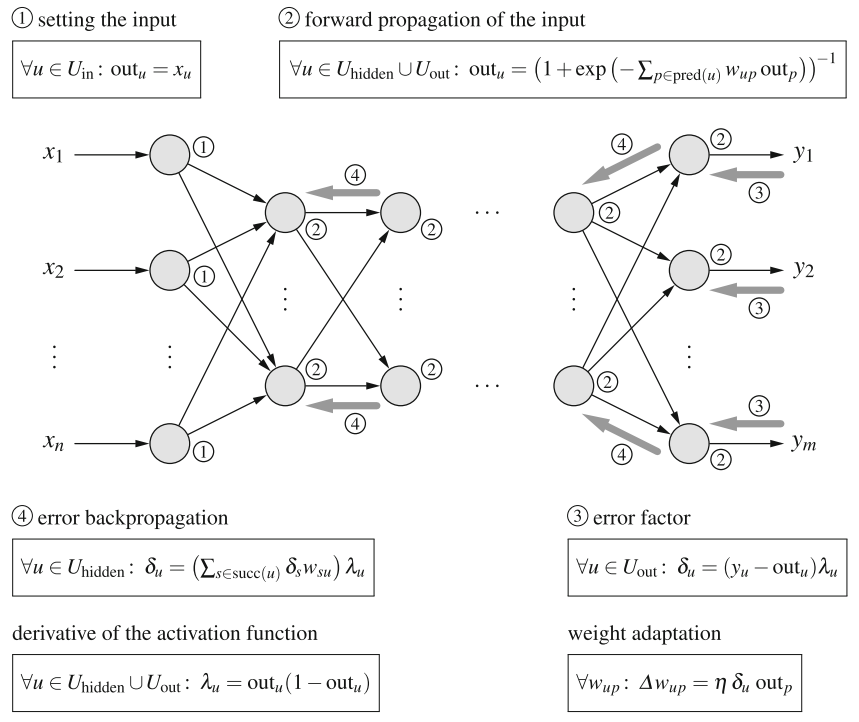
\includegraphics[scale=0.5]{images/error_backpropagation.png}
    \caption{Schematized structure of the error backpropagation process}
    \label{fig:error_backpropagation}
\end{figure}

We assume that the activation functions is a \textit{logistic function} for each neuron
$u\in U_{(hidden)}\cup U_{(out)}$, except for the input neurons.
\begin{enumerate}
    \item Apply the input at the input neurons that is returned without modifications
          at the subsequent first hidden layer.
    \item We compute for each neuron of the subsequent layers the weighted sum of the
          inputs and we apply at the result the logistic function, producing the output
          that will be propagated in all the network until the terminal neurons.
    \item Compute the difference between the desired output and the actual output. since
          it is possible to invert the logistic function $f_{(act)}$, we can know which was
          the input (error) that has induced that particular error ($\delta_u$).
    \item Now that we have transformed the error of the output variable $out_u$ in
          the error of the input variable $net_u$, we can distribute the error (with the correction)
          in a proportional way back to previous neuron, we back propagate the error until the
          input neurons.
\end{enumerate}

We have to say that given the shape of the logistic function the error can disappear
completely, since the gradient will approximate more the \textbf{null vector} the
more it will be near the zero.

The weight adaptation is performed by the following formula (this tells me how to perform the correction):
$$\forall w_{up}:\delta w_{up}=\eta \delta_u out_p$$

If you initialize the \textit{learning rate} $\eta$ with a too high value instead
of descending the curve we risk to jump from a \textit{"peak"} of the function to another,
without ever converging to the minimum. Furthermore, it is not all certain that the minimum
reached in this way is the global minimum of the function.

A solution to the problem could consist in \textit{repeating} the learning, initializing
the system with a different configuration of weights and threshold, and then choice
at the end which configuration result in the better minimum.
\paragraph{Negation example}
For example let's consider the negation $\lnot x$, there is a two-layer perceptron for this function.
\begin{figure}[H]
    \centering
    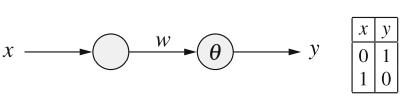
\includegraphics[scale=0.5]{images/2_per_neg.png}
    \caption{Two-layer perceptron with single input and training examples for the negation}
\end{figure}

\begin{figure}[H]
    \centering
    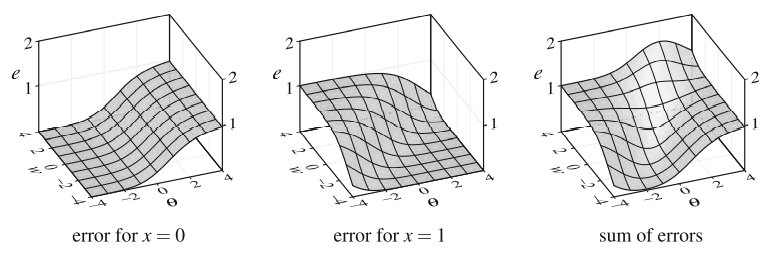
\includegraphics[scale=0.55]{images/squared_errors.png}
    \caption{Squared errors for computing the negation by using a logic activation function}
\end{figure}

From a numeric point of view, this procedure won't allow us to reach really the minimum, we will ahave some
residual errors due to the computation of the various parameters (this will change according to the
process we are adopting).

\subsubsection{Variant of Gradient Descend}
The variant aim to change the \textbf{learning rate} and the \textbf{length of the learning step}.

\begin{itemize}
    \item \textit{Manhattan training}, taking just the sign of the gradient, very fast but you may not reach
          the optimum.

    \item \textit{Flat spot elimination}, it tries to limit the culling of the step length when we get near a
          function plateau by "lifting" artificially the derivative of the function in that point.

    \item \textit{Momentum term}, at each successive step we add to the gradient a fraction of the previous
          with changed weights, so that we can have a sort of memory of how fast it changes respect to the past.

    \item \textit{Self-adaptive error backpropagation}, i allow to each parameter to have a different
          learning rate, in this way we can have a grain fine control respect to the characteristic of the single parameter.

    \item \textit{Resilient error backpropagation}, it's a combination of the Manhattan variation with the Self-adaptive.

    \item \textit{Quick propagation}, instead of using the gradient i approximate the function with a parable and i
          jump directly to the peak of this one.

    \item \textit{Weight decay}, reduces the weights for avoiding to remain trapped in an already saturated region
          (avoiding too big weights to keep stuck neurons).
\end{itemize}

\subsection{Number of hidden neurons}
For a single hidden layer the following rule of thumb is popular (take as granted):
$$\text{Number of hidden neurons} = \left(\frac{\text{number of inputs}+\text{number of outputs}}{2}\right)$$
The problem is that if we have to few neurons in the hidden layer, we will not be able to achieve a good approximation
the function that we need to approximate. We have not enough parameters, this behavior is called \textbf{underfitting}.

On the contrary, if we have very large hidden layers we have many neurons, we have many many parameters to train and this may force the
NN to learn the examples to much, and this will focus the network on this examples only, we lose the ability of
generalizing the desired behavior, this is called \textbf{overfitting}.
\begin{figure}[H]
    \centering
    \includegraphics[scale=0.6]{images/overfitting.png}
    \caption{The blue curve fits the data points perfectly, not a good model}
\end{figure}
For example, the NN learned perfectly the blue line to pass exactly in the points, but this is not what we
want to have. Now we can't generalize the abstract view of the black line (too many parameters).

\textit{What we need to do in order to understand when we have good quality for our learning?} Follow, the
next subsection.
\subsection{Cross validation}
In order to understand if we have a good quality for our learning we need to
randomly split our data sets in two parts:
\begin{itemize}
    \item Training set: used for the training.
    \item Validation set: used for checking the quality of the result.
\end{itemize}
This will allow us to see (by using the validation set) if the training makes the NN overfitting the configuration or
not, if the error that we have is still reasonable low, we have a good quality of the learning
(we still can do good generalization), viceversa we have a bad learning quality.

We can do the splitting in two ways:
\begin{itemize}
    \item \textbf{Cross validation}: splits randomly the data in two subsets (for training and validation),
          we train the MLP with different numbers of hidden neurons on the training data and evaluate them on the
          validation data. Then you repeat the split of the data and the training-evaluation many times and average the
          results. At the end you choose the number of hidden neurons with the best average error.

    \item \textbf{N-fold cross validation}: the data is split in $n$ subsets (called \textit{folds}) of
          about equal size. The relative frequency of the output values in the folds represent as well as possible the
          relative frequencies of these values in the data set as a whole (\textbf{stratification}). Out of these
          $n$ data subsets, $n$ pairs of training and validation data set are formed by using $1$ fold as a validation
          and $n-1$ folds for training.
\end{itemize}

randomly the data in two subsets for training and validation (\textbf{cross validation}) and we can repeat this splitting in different
phases and at the end we can compare the. or we can split the data set in N-folds (\textbf{N-folds validation})
and then use the various $n$ subsets for training and $n-1$ subsets for validation, in this way we can use
most of the example for training instead of validation.

The \textbf{stopping criterion} is also very important, we stop the training when the validation
error is sufficient low.

\subsubsection{Sensitivity analysis}
Sensitivity of the NN to the various parameters that we have, the variations that we may have to the
various parameters influences the behavior of our NN. We want understand how muc hthe learning applied to the NN
is really independent from the behavior of the NN.

This is important to understand how much is generalizable the behavior of our NN.

This is a problem for MLP, when we perform the learning (supervised or unsupervised), basically we have a
data set presented to the NN and then the learning algorithm adjust the parameters in ordered to find the
desired behavior of the NN.

In our hands we have an algorithm, but we don't have an understanding of the why the parameter
are configured in this way. We are trying to give an explanation of why a NN is configured in a specific way,
this is actually field of research (we still don't have a rational idea).

For the sensitivity analysis which is part of this understanding, we want to answer this question: \textit{How much
    the output of each neuron is changing if we change the data set for training}
(still describing the desired behavior)\textit{?}
So essentially, which inputs the output(s) react(s) most sensitively, it hints about which inputs aren't needed
and may be discarded.

The approach consists in determine the change of ourput relative to the change of input:
$$\forall u\in U_{in}:
    s(u)=\frac{1}{|L_{fixed}|} \sum_{l\in L_{fixed}} \sum_{v\in U_{out}} \frac{\partial out_v^{(l)}}{\partial ext_u^{(l)}}$$

\subsection{Deep learning}
A modern approach to MLP called \textbf{Deep learning}, with MLP we can approximate any continuos integrable
function, but we have in general a pretty large hidden layer. First problem, \textit{what we can do to
    simplify the structure?} The second problem, with MLP we have to know the characteristic of the data which are
relevant to pick the important data to configure the NN.

It has been experimented that adding $1$ or $2$ more layers helps to have a concise NN but with
the same characteristic of a MLP with a large number of neurons in the hidden layers.

The deep learning network is basically a MLP, but with a difference: What we want to do it consists
in not having any type of knowledge about the problem and try to force the NN to configure itself with
a limited and small number of neurons.

For example, let's consider the $n$-bit parity function, which output $1$ if the $n$-bit word is even,
or viceversa $0$. If we want to use an MLP with only one hidden layer, which has $2^{n-1}$ neurons, the number
of hidden neurons grows \textbf{exponentially} with the number of inputs. This because the function is a
disjunction of  $2^{n-1}$ conjunctions.
\begin{figure}
    \centering
    \includegraphics[scale=0.5]{images/nbit_parity.png}
    \caption{$n$-bit parity function}
\end{figure}
Instead if we use \textbf{multiple} hidden layers, the \textbf{linear growth} is possible (respect to the
input). This finding bring to the developing of \textit{deep learning}, where the \textit{"depth"} is the
one given by the longest path which separates the input neurons from the output neurons.

The rational is to allow a greater deepness of the network in change of better performance in construction
and computation of the NN. The deep learning bring some downsides:
\begin{itemize}
    \item \textit{Overfitting}: the increases of neurons given from the extra hidden layers can multiply
          the parameters in a disproportional way.
    \item \textit{Vanishing gradient}: during the propagation of the error the gradient will get reduced
          until the vanishing.
\end{itemize}

Some solutions to the overfitting issue:
\begin{itemize}
    \item \textit{Weight decay}: set a maximum limit to the values which can assume weights
          this for preventing an adjustment too much dependent from the data set.
    \item \textit{Sparsity constraint}: introducing some limit to the number of neurons of the
          hidden layers, or limiting the number of the active neurons.
    \item \textit{Dropout training}: some neurons of the hidden layers are omtitted during the
          evolution of the network.
\end{itemize}

While the issue of the vanishing gradient is given by the fact that the activation function it's a
logistic function, which derivative reach at max the value of $\frac{1}{4}$. As consequence of this
the propagation of the error to a previous layer adds a value, often smaller than $1$, and in this
way reducing the gradient.

A solution consists in editing slightly the activation function in a way that will be always increasing.
Some candidates for that are the \textit{ramp function} and the \textit{softplus function}.
\begin{figure}
    \centering
    \includegraphics[scale=0.5]{images/ramp_softplus.png}
    \caption{Ramp function and softplus function}
\end{figure}
A totally different approach consist in building the network \textit{"layer by layer"}. A much used
technique consists in think at the NN like a stack of \textit{autoencoder}. An autoencoder is an MLP
which maps the input inside an approximation, using an hidden layers of less dimensions. The
hidden layer works like an \textit{encoder} by encoding the input in a internal representation
which will be decoded to the output layer. The autoencoder, has only one layer, it doesn't suffer
about the same limitation and can be traversed normally from the backpropagation.

A problem with this approach is that if there are a lot of neurons in hidden layer as much are in
the input layer we are going to propagate with less adjustments, and without the autoencoder
extracting any knowledge from the data.

There are three possible solutions:
\begin{itemize}
    \item \textit{Sparse autoencoder}: provide to use a much smaller number of neurons inside the
          hidden layers, respect to the input layers. The autoencoder will be forced to extract from
          the input some features instead of just propagating the data.

    \item \textit{Sparse activation scheme}: in a similar way for avoiding the overfitting, we
          decide to \textit{"shutdown"} some neurons during the computation.

    \item \textit{De-noising autoencoder}: we add randomly some noise to the input.
\end{itemize}

For obtaining an MLP with multiple layers we combine differente autoencoder. Initially we start by
training just one autoencoder. At that time you remove the decoder and you preserve only the internal layer.
You use the data processed from this autoencoder for training the second, and so on until you
reach a satisfiable number of layers.
\begin{figure}
    \centering
    \includegraphics[scale=0.5]{images/autoencoder_decoder.png}
    \caption{Autoencoder and autoencoder with the decoder removed}
\end{figure}
MLP constructed in this way are really efficient at recognizing with success hand written numbers. If
we would want to use similar NN for a more broad class of applications, like, for example, the
feature recognized by the internal layers are not located in a specific portion of the image, we would
need to use a CNN (\textit{Convolutional Neural Network}, next topic). This architecture is inspired
by the working of the human retina, where the neurons used for the perception has a receptive field,
or in other words, a limited region where they can answer to stimulus.

This is simulated inside the CNN by connecting the neurons of the first layer just to some neurons
of the input. The weights are partitioned in a way that partial networks can be evaluated  from
different prospective of the image.

During the computation it will proceed by moving the receptive field on the totality of the image. As
result you will obtain a convolution of the weight matrix with the input image.

\subsection{Radial Basis Function Networks}
This is another NN model, we have a special type of structure for the neurons and a special approach
for information we are collecting from images (typically).

I have a 3-layered feed forward network, where the activation function of the hidden layer is a \textit{
    Radial Basis Function} (RBF).

An RBF is a function which try to point out what is relevant in a very specific area of the information
we are observing (an image), and tries to diminish what is in the surrounding area. So it will focus on
relevant part of the image where we want to understand the contents.

In this kind of NN we have a set of values for various inputs, we represent this with a vector, we have
for example a three dimensional space, where each value represent the input. What i'm considering as input
of the hidden layer is the difference between this vector and the weight vector, which is the distance
between the vectors.
\begin{figure}[H]
    \centering
    \includegraphics[scale=0.5]{images/rbf.png}
    \caption{Distance between $\vec{w}$ and $\vec{in}_{u}$}
\end{figure}
There are different families of distances, we typical consider the \textbf{Minkowski Family}, which are
distances defined in general by this formula:
$$d_k(\vec{x},\vec{y})=\left(\sum_{i=1}^n |x_i-y_i|^k\right)^{\frac{1}{k}}$$
\begin{itemize}
    \item $k=1$: Manhattan distance.
    \item $k=2$: Euclidean distance.
    \item $k\rightarrow\infty$: Maximum distance.
\end{itemize}

\begin{figure}[H]
    \centering
    \includegraphics[scale=0.5]{images/mknowski.png}
    \caption{Manhattan, Euclidean and Maximum}
\end{figure}

The RBF has an activation function in the output layer which is \textbf{linear}. Differently, the
hidden layer has an activation function which is a \textbf{radial function}. A radial function
decreases from $0$ to $\infty$ in a monotonically way.

$$f:\mathbb{R}_0^+\rightarrow[0,1]\text{ with }f(0)=1\text{ and }\lim_{x\rightarrow\infty}f(x)=0$$
The size of the \textit{catchment region} of the function is defined by
the \textbf{reference radius} $\sigma$, the bigger is the $\sigma$ the bigger
is the area observed by the neuron. The various parameters and the shape of the function
determine the width of this radius. The radial activation function are typically shaped in this way:
\begin{figure}[H]
    \centering
    \includegraphics[scale=0.4]{images/radial_functions.png}
    \caption{Radial activation functions}
\end{figure}
As example, let's apply an RBFN for simulating the boolean conjunction $x_1\land x_2$.
When i'm around the black point, the input is $(1,1)$, what we want to do is creating a circle
around that area where the output is $1$ (significant information to extract).

Another approach could consist in considering a RBF in the opposite way, where the interesting
data is outside the circle.
\begin{figure}[H]
    \centering
    \includegraphics[scale=0.5]{images/RBFN.png}
    \caption{RBFN for conjunction}
\end{figure}
Another example is with the bi-implication $x_1\longleftrightarrow x_2$:
\begin{figure}[H]
    \centering
    \includegraphics[scale=0.4]{images/RBFN_bi.png}
    \caption{RBFN for bi-implication}
\end{figure}

\paragraph{Function approximation}
We have two neurons focusing on the relevant part of the domain, the rest will be $0$, and by merging
this two information you will get the bi-implication. In general an RBFN as the same expressive
power of an MLP, and it can be saw as an universal approximator (can approximate any Riemann integrable
function) with a small arbitrary error.

The process is the same of the other NN, the function will get approximated with a step function that
can be computed easily by a RBF if we define that as the weighted sum of rectangular functions.
\begin{figure}[H]
    \centering
    \includegraphics[scale=0.4]{images/scale_func.png}
\end{figure}
Each pulse can be represented by a neuron of a RBFN:
\begin{figure}
    \centering
    \includegraphics[scale=0.5]{images/nn_funcapprox_rbfn.png}
    \caption{RBFN for the approximation, using the step function}
\end{figure}
The approximation can be enhanced by increasing the number of points where the function is
being evaluated. Furthermore, if instead of using the rectangular function, we
use the Gaussian we obtain more "soft" transitions, avoiding big jumps (like for the MLP).
\begin{figure}[H]
    \centering
    \includegraphics[scale=0.4]{images/gaussian_rbfn.png}
    \caption{RBFN for the approximation, using the Gaussian function}
\end{figure}

\subsection{Training RBFN}
The principle is always the same, having in mind the \textit{minimization} of the final error,
but the problem here is \textit{how we can decline this by taking into account the
    specific structure of this neurons?}
With the others ANN the initialization fase was trivial, because you just had to
select some random values, instead with RBFN the same approach conduce to suboptimal
results.

Let's consider the special caso of \textbf{simple radial basis function network}, which is
a partial view of the general structure of a RBFN, where each training example is associated
with a proper radial function.

We want to apply a \textbf{fixed learning task} $L_{fixed}?\{l_1,...,l_m\}$ with
$m$ training patterns $l=(\vec{l}^{(l)},\vec{o}^{(l)})$ composed by input and desired outputs.

Let's define the vector of associated weights to the neuron $v_k$, with $k=1,...,m$ (one
for each training pattern):
$$\forall k\in\{1,...,m\}\vec{w}_{v_k}=\vec{i}^{l_k}$$
Assuming a Gaussian activation function, the radius $\sigma_k$ is initialized according to this heuristic:
$$\forall k\in\{1,...,m\}:\sigma_k = \frac{d_{max}}{\sqrt{2m}}$$
Where $d_{max}$ is the maximum distance between the input vectors. This choice allow to center the various
Gaussians in such a way that them doesn't overlap each other, instead they will distributes in an ordered way
respect to the input space.
$$d_{max}=max\underset{l_j,l_k\in L_{fixed}}{d\left(\vec{l}^{(l_j)},\vec{l}^(l_k)\right)}$$
For what concerns the weights of the output neurons, they get calculated with the following
function:
$$\forall u:\sum_{k=1}^{m}w_{u_k}out_{u_k}-\theta=o_u$$
By using $\theta=0$, we will get that the previous equation will be:
$$\textbf{A}\cdot\vec{w}_u=\vec{o}_u$$
Where $\textbf{A}$ is the $m\times m$ matrix that got has components the various output of the neurons
in the hidden layer. If the matrice $\textbf{A}$ has the complete rank, we can invert that and
compute the weight vector:
$$\vec{w}_u=\textbf{A}^{-1}\cdot\vec{o}_u$$
\end{document}